\documentclass[twoside]{book}

% Packages required by doxygen
\usepackage{fixltx2e}
\usepackage{calc}
\usepackage{doxygen}
\usepackage[export]{adjustbox} % also loads graphicx
\usepackage{graphicx}
\usepackage[utf8]{inputenc}
\usepackage{makeidx}
\usepackage{multicol}
\usepackage{multirow}
\PassOptionsToPackage{warn}{textcomp}
\usepackage{textcomp}
\usepackage[nointegrals]{wasysym}
\usepackage[table]{xcolor}

% Font selection
\usepackage[T1]{fontenc}
\usepackage[scaled=.90]{helvet}
\usepackage{courier}
\usepackage{amssymb}
\usepackage{sectsty}
\renewcommand{\familydefault}{\sfdefault}
\allsectionsfont{%
  \fontseries{bc}\selectfont%
  \color{darkgray}%
}
\renewcommand{\DoxyLabelFont}{%
  \fontseries{bc}\selectfont%
  \color{darkgray}%
}
\newcommand{\+}{\discretionary{\mbox{\scriptsize$\hookleftarrow$}}{}{}}

% Page & text layout
\usepackage{geometry}
\geometry{%
  a4paper,%
  top=2.5cm,%
  bottom=2.5cm,%
  left=2.5cm,%
  right=2.5cm%
}
\tolerance=750
\hfuzz=15pt
\hbadness=750
\setlength{\emergencystretch}{15pt}
\setlength{\parindent}{0cm}
\setlength{\parskip}{3ex plus 2ex minus 2ex}
\makeatletter
\renewcommand{\paragraph}{%
  \@startsection{paragraph}{4}{0ex}{-1.0ex}{1.0ex}{%
    \normalfont\normalsize\bfseries\SS@parafont%
  }%
}
\renewcommand{\subparagraph}{%
  \@startsection{subparagraph}{5}{0ex}{-1.0ex}{1.0ex}{%
    \normalfont\normalsize\bfseries\SS@subparafont%
  }%
}
\makeatother

% Headers & footers
\usepackage{fancyhdr}
\pagestyle{fancyplain}
\fancyhead[LE]{\fancyplain{}{\bfseries\thepage}}
\fancyhead[CE]{\fancyplain{}{}}
\fancyhead[RE]{\fancyplain{}{\bfseries\leftmark}}
\fancyhead[LO]{\fancyplain{}{\bfseries\rightmark}}
\fancyhead[CO]{\fancyplain{}{}}
\fancyhead[RO]{\fancyplain{}{\bfseries\thepage}}
\fancyfoot[LE]{\fancyplain{}{}}
\fancyfoot[CE]{\fancyplain{}{}}
\fancyfoot[RE]{\fancyplain{}{\bfseries\scriptsize Generated by Doxygen }}
\fancyfoot[LO]{\fancyplain{}{\bfseries\scriptsize Generated by Doxygen }}
\fancyfoot[CO]{\fancyplain{}{}}
\fancyfoot[RO]{\fancyplain{}{}}
\renewcommand{\footrulewidth}{0.4pt}
\renewcommand{\chaptermark}[1]{%
  \markboth{#1}{}%
}
\renewcommand{\sectionmark}[1]{%
  \markright{\thesection\ #1}%
}

% Indices & bibliography
\usepackage{natbib}
\usepackage[titles]{tocloft}
\setcounter{tocdepth}{3}
\setcounter{secnumdepth}{5}
\makeindex

% Hyperlinks (required, but should be loaded last)
\usepackage{ifpdf}
\ifpdf
  \usepackage[pdftex,pagebackref=true]{hyperref}
\else
  \usepackage[ps2pdf,pagebackref=true]{hyperref}
\fi
\hypersetup{%
  colorlinks=true,%
  linkcolor=blue,%
  citecolor=blue,%
  unicode%
}

% Custom commands
\newcommand{\clearemptydoublepage}{%
  \newpage{\pagestyle{empty}\cleardoublepage}%
}

\usepackage{caption}
\captionsetup{labelsep=space,justification=centering,font={bf},singlelinecheck=off,skip=4pt,position=top}

%===== C O N T E N T S =====

\begin{document}

% Titlepage & ToC
\hypersetup{pageanchor=false,
             bookmarksnumbered=true,
             pdfencoding=unicode
            }
\pagenumbering{alph}
\begin{titlepage}
\vspace*{7cm}
\begin{center}%
{\Large Study of multiple Heat Diffusion schemes \\[1ex]\large 1.\+0.\+0 }\\
\vspace*{1cm}
{\large Generated by Doxygen 1.8.14}\\
\end{center}
\end{titlepage}
\clearemptydoublepage
\pagenumbering{roman}
\tableofcontents
\clearemptydoublepage
\pagenumbering{arabic}
\hypersetup{pageanchor=true}

%--- Begin generated contents ---
\chapter{Hierarchical Index}
\section{Class Hierarchy}
This inheritance list is sorted roughly, but not completely, alphabetically\+:\begin{DoxyCompactList}
\item \contentsline{section}{Solver}{\pageref{classSolver}}{}
\begin{DoxyCompactList}
\item \contentsline{section}{Analytic}{\pageref{classAnalytic}}{}
\item \contentsline{section}{Crank\+Nicolson}{\pageref{classCrankNicolson}}{}
\item \contentsline{section}{Dufort\+Frankel}{\pageref{classDufortFrankel}}{}
\item \contentsline{section}{Laasonen}{\pageref{classLaasonen}}{}
\item \contentsline{section}{Richardson}{\pageref{classRichardson}}{}
\end{DoxyCompactList}
\item vector\begin{DoxyCompactList}
\item \contentsline{section}{Matrix}{\pageref{classMatrix}}{}
\item \contentsline{section}{Vector}{\pageref{classVector}}{}
\end{DoxyCompactList}
\end{DoxyCompactList}

\chapter{Class Index}
\section{Class List}
Here are the classes, structs, unions and interfaces with brief descriptions\+:\begin{DoxyCompactList}
\item\contentsline{section}{\mbox{\hyperlink{classAnalytic}{Analytic}} }{\pageref{classAnalytic}}{}
\item\contentsline{section}{\mbox{\hyperlink{classCrankNicolson}{Crank\+Nicolson}} }{\pageref{classCrankNicolson}}{}
\item\contentsline{section}{\mbox{\hyperlink{classDufortFrankel}{Dufort\+Frankel}} }{\pageref{classDufortFrankel}}{}
\item\contentsline{section}{\mbox{\hyperlink{classLaasonen}{Laasonen}} }{\pageref{classLaasonen}}{}
\item\contentsline{section}{\mbox{\hyperlink{classMatrix}{Matrix}} }{\pageref{classMatrix}}{}
\item\contentsline{section}{\mbox{\hyperlink{classRichardson}{Richardson}} }{\pageref{classRichardson}}{}
\item\contentsline{section}{\mbox{\hyperlink{classSolver}{Solver}} }{\pageref{classSolver}}{}
\item\contentsline{section}{\mbox{\hyperlink{classVector}{Vector}} }{\pageref{classVector}}{}
\end{DoxyCompactList}

\chapter{Class Documentation}
\hypertarget{classAnalytic}{}\section{Analytic Class Reference}
\label{classAnalytic}\index{Analytic@{Analytic}}
Inheritance diagram for Analytic\+:\begin{figure}[H]
\begin{center}
\leavevmode
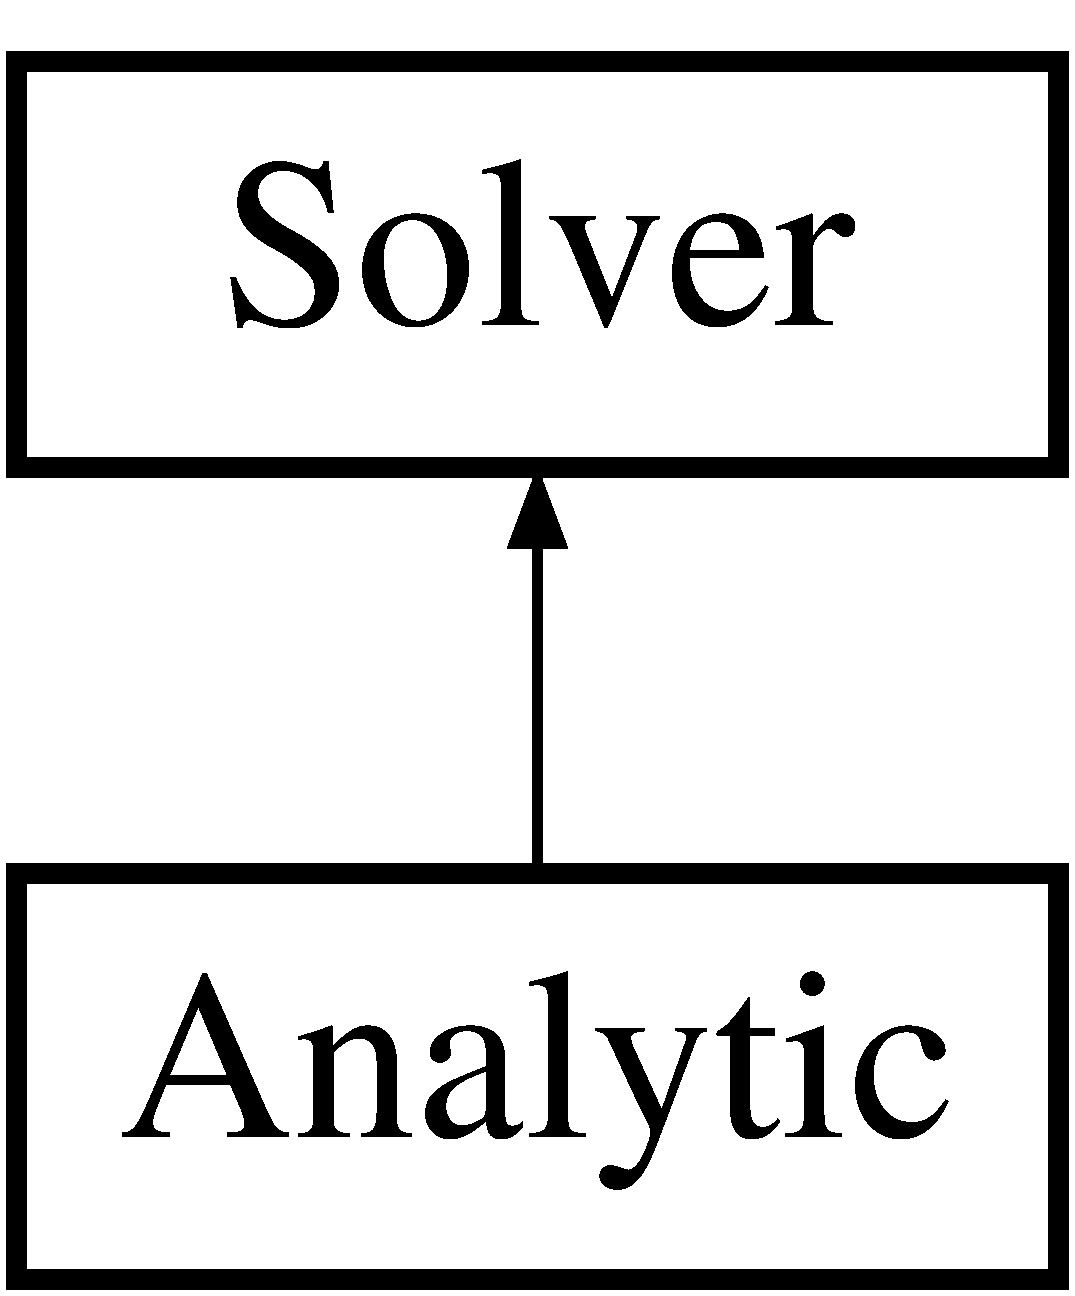
\includegraphics[height=2.000000cm]{classAnalytic}
\end{center}
\end{figure}
\subsection*{Public Member Functions}
\begin{DoxyCompactItemize}
\item 
\mbox{\hyperlink{classAnalytic_a22578fb39f290a77a0a9bacfe85c6406}{Analytic}} (double dx, double dt, double L, double T, double D, double Tsur, double Tin)
\item 
virtual \mbox{\hyperlink{classMatrix}{Matrix}} \mbox{\hyperlink{classAnalytic_aaa59a993d9c1a9b9c5b581f8f3e9c5b3}{compute\+Solution}} ()
\end{DoxyCompactItemize}
\subsection*{Additional Inherited Members}


\subsection{Constructor \& Destructor Documentation}
\mbox{\Hypertarget{classAnalytic_a22578fb39f290a77a0a9bacfe85c6406}\label{classAnalytic_a22578fb39f290a77a0a9bacfe85c6406}} 
\index{Analytic@{Analytic}!Analytic@{Analytic}}
\index{Analytic@{Analytic}!Analytic@{Analytic}}
\subsubsection{\texorpdfstring{Analytic()}{Analytic()}}
{\footnotesize\ttfamily Analytic\+::\+Analytic (\begin{DoxyParamCaption}\item[{double}]{dx,  }\item[{double}]{dt,  }\item[{double}]{L,  }\item[{double}]{T,  }\item[{double}]{D,  }\item[{double}]{Tsur,  }\item[{double}]{Tin }\end{DoxyParamCaption})}

Construcs an analyic object 
\begin{DoxyParams}{Parameters}
{\em dx} & double. distance between two space steps \\
\hline
{\em dt} & double. time between two time steps \\
\hline
{\em L} & double. width of the 1D material to consider \\
\hline
{\em T} & double. Total time of the considerated problem \\
\hline
{\em D} & double. Diffusion coefficient of the material \\
\hline
{\em Tsur} & double. The temperature that will be applied on the boundaries of the material \\
\hline
{\em Tin} & double. The initial temperature of the material \\
\hline
\end{DoxyParams}


\subsection{Member Function Documentation}
\mbox{\Hypertarget{classAnalytic_aaa59a993d9c1a9b9c5b581f8f3e9c5b3}\label{classAnalytic_aaa59a993d9c1a9b9c5b581f8f3e9c5b3}} 
\index{Analytic@{Analytic}!compute\+Solution@{compute\+Solution}}
\index{compute\+Solution@{compute\+Solution}!Analytic@{Analytic}}
\subsubsection{\texorpdfstring{compute\+Solution()}{computeSolution()}}
{\footnotesize\ttfamily \mbox{\hyperlink{classMatrix}{Matrix}} Analytic\+::compute\+Solution (\begin{DoxyParamCaption}{ }\end{DoxyParamCaption})\hspace{0.3cm}{\ttfamily [virtual]}}

Compute the solution and return it. This method is the analytical solution of the heat diffusion equation problem \begin{DoxyReturn}{Returns}
\mbox{\hyperlink{classMatrix}{Matrix}}. The computed matrix, can also be accesed through \mbox{\hyperlink{classSolver_aafe88ce4130c001052e5d93c1681f90f}{get\+Computed\+Solution()}} 
\end{DoxyReturn}
\begin{DoxySeeAlso}{See also}
\mbox{\hyperlink{classSolver_aafe88ce4130c001052e5d93c1681f90f}{get\+Computed\+Solution()}} 
\end{DoxySeeAlso}


Implements \mbox{\hyperlink{classSolver_a0f4ecfaed825407019995b5176e25748}{Solver}}.



The documentation for this class was generated from the following files\+:\begin{DoxyCompactItemize}
\item 
Analytic.\+h\item 
Analytic.\+cpp\end{DoxyCompactItemize}

\hypertarget{classCrankNicolson}{}\section{Crank\+Nicolson Class Reference}
\label{classCrankNicolson}\index{Crank\+Nicolson@{Crank\+Nicolson}}
Inheritance diagram for Crank\+Nicolson\+:\begin{figure}[H]
\begin{center}
\leavevmode
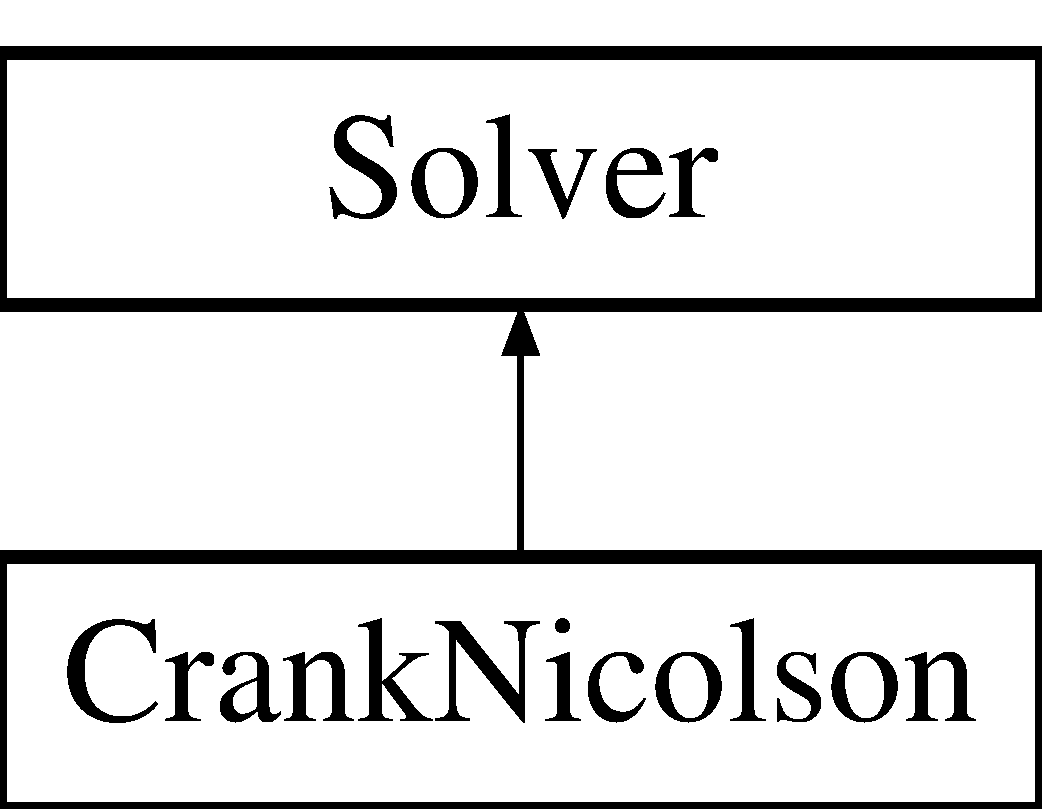
\includegraphics[height=2.000000cm]{classCrankNicolson}
\end{center}
\end{figure}
\subsection*{Public Member Functions}
\begin{DoxyCompactItemize}
\item 
\mbox{\hyperlink{classCrankNicolson_a722060b8060158412b131179a1c484ce}{Crank\+Nicolson}} (double dx, double dt, double L, double T, double D, double Tsur, double Tin)
\item 
virtual \mbox{\hyperlink{classMatrix}{Matrix}} \mbox{\hyperlink{classCrankNicolson_a94af3b8a56ef40966ea2ccd2629c2eb2}{compute\+Solution}} ()
\end{DoxyCompactItemize}
\subsection*{Additional Inherited Members}


\subsection{Constructor \& Destructor Documentation}
\mbox{\Hypertarget{classCrankNicolson_a722060b8060158412b131179a1c484ce}\label{classCrankNicolson_a722060b8060158412b131179a1c484ce}} 
\index{Crank\+Nicolson@{Crank\+Nicolson}!Crank\+Nicolson@{Crank\+Nicolson}}
\index{Crank\+Nicolson@{Crank\+Nicolson}!Crank\+Nicolson@{Crank\+Nicolson}}
\subsubsection{\texorpdfstring{Crank\+Nicolson()}{CrankNicolson()}}
{\footnotesize\ttfamily Crank\+Nicolson\+::\+Crank\+Nicolson (\begin{DoxyParamCaption}\item[{double}]{dx,  }\item[{double}]{dt,  }\item[{double}]{L,  }\item[{double}]{T,  }\item[{double}]{D,  }\item[{double}]{Tsur,  }\item[{double}]{Tin }\end{DoxyParamCaption})}

Construcs a solver of the problem using Crank-\/\+Nicolson method 
\begin{DoxyExceptions}{Exceptions}
{\em invalid\+\_\+argument} & (\char`\"{}dx should be positive\char`\"{}) \\
\hline
{\em invalid\+\_\+argument} & (\char`\"{}dt should be positive\char`\"{}) \\
\hline
{\em invalid\+\_\+argument} & (\char`\"{}\+L should be positive\char`\"{}) \\
\hline
{\em invalid\+\_\+argument} & (\char`\"{}\+T should be positive\char`\"{}) \\
\hline
{\em invalid\+\_\+argument} & (\char`\"{}\+L should be equal or larger than dx\char`\"{}) \\
\hline
{\em invalid\+\_\+argument} & (\char`\"{}\+T should be equal or larger than dt\char`\"{}) \\
\hline
\end{DoxyExceptions}

\begin{DoxyParams}{Parameters}
{\em dx} & double. distance between two space steps \\
\hline
{\em dt} & double. time between two time steps \\
\hline
{\em L} & double. width of the 1D material to consider \\
\hline
{\em T} & double. Total time of the considerated problem \\
\hline
{\em D} & double. Diffusion coefficient of the material \\
\hline
{\em Tsur} & double. The temperature that will be applied on the boundaries of the material \\
\hline
{\em Tin} & double. The initial temperature of the material \\
\hline
\end{DoxyParams}


\subsection{Member Function Documentation}
\mbox{\Hypertarget{classCrankNicolson_a94af3b8a56ef40966ea2ccd2629c2eb2}\label{classCrankNicolson_a94af3b8a56ef40966ea2ccd2629c2eb2}} 
\index{Crank\+Nicolson@{Crank\+Nicolson}!compute\+Solution@{compute\+Solution}}
\index{compute\+Solution@{compute\+Solution}!Crank\+Nicolson@{Crank\+Nicolson}}
\subsubsection{\texorpdfstring{compute\+Solution()}{computeSolution()}}
{\footnotesize\ttfamily \mbox{\hyperlink{classMatrix}{Matrix}} Crank\+Nicolson\+::compute\+Solution (\begin{DoxyParamCaption}{ }\end{DoxyParamCaption})\hspace{0.3cm}{\ttfamily [virtual]}}

Compute the solution and return it. This method is the Crank-\/\+Nicolson method applied to the heat diffusion equation problem \begin{DoxyReturn}{Returns}
\mbox{\hyperlink{classMatrix}{Matrix}}. The computed matrix, can also be accesed through \mbox{\hyperlink{classSolver_aafe88ce4130c001052e5d93c1681f90f}{get\+Computed\+Solution()}} 
\end{DoxyReturn}
\begin{DoxySeeAlso}{See also}
\mbox{\hyperlink{classSolver_aafe88ce4130c001052e5d93c1681f90f}{get\+Computed\+Solution()}} 
\end{DoxySeeAlso}


Implements \mbox{\hyperlink{classSolver_a0f4ecfaed825407019995b5176e25748}{Solver}}.



The documentation for this class was generated from the following files\+:\begin{DoxyCompactItemize}
\item 
Crank\+Nicolson.\+h\item 
Crank\+Nicolson.\+cpp\end{DoxyCompactItemize}

\hypertarget{classDufortFrankel}{}\section{Dufort\+Frankel Class Reference}
\label{classDufortFrankel}\index{Dufort\+Frankel@{Dufort\+Frankel}}
Inheritance diagram for Dufort\+Frankel\+:\begin{figure}[H]
\begin{center}
\leavevmode
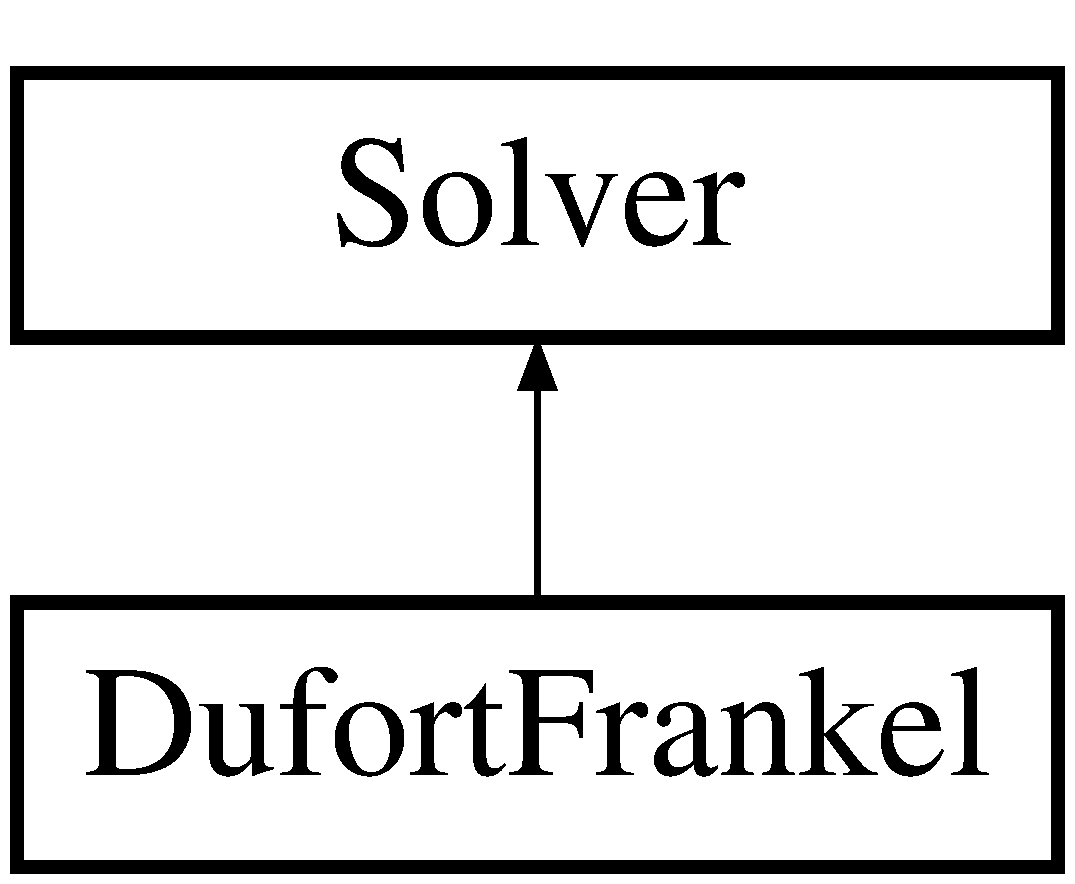
\includegraphics[height=2.000000cm]{classDufortFrankel}
\end{center}
\end{figure}
\subsection*{Public Member Functions}
\begin{DoxyCompactItemize}
\item 
\mbox{\hyperlink{classDufortFrankel_ab0c732f705d9b0aa1df228670a74b651}{Dufort\+Frankel}} (double dx, double dt, double L, double T, double D, double Tsur, double Tin)
\item 
virtual \mbox{\hyperlink{classMatrix}{Matrix}} \mbox{\hyperlink{classDufortFrankel_aad9f0443398cd3f32b44739c1133fa94}{compute\+Solution}} ()
\end{DoxyCompactItemize}
\subsection*{Additional Inherited Members}


\subsection{Constructor \& Destructor Documentation}
\mbox{\Hypertarget{classDufortFrankel_ab0c732f705d9b0aa1df228670a74b651}\label{classDufortFrankel_ab0c732f705d9b0aa1df228670a74b651}} 
\index{Dufort\+Frankel@{Dufort\+Frankel}!Dufort\+Frankel@{Dufort\+Frankel}}
\index{Dufort\+Frankel@{Dufort\+Frankel}!Dufort\+Frankel@{Dufort\+Frankel}}
\subsubsection{\texorpdfstring{Dufort\+Frankel()}{DufortFrankel()}}
{\footnotesize\ttfamily Dufort\+Frankel\+::\+Dufort\+Frankel (\begin{DoxyParamCaption}\item[{double}]{dx,  }\item[{double}]{dt,  }\item[{double}]{L,  }\item[{double}]{T,  }\item[{double}]{D,  }\item[{double}]{Tsur,  }\item[{double}]{Tin }\end{DoxyParamCaption})}

Construcs a solver of the problem using Du\+Fort-\/\+Frankel method 
\begin{DoxyExceptions}{Exceptions}
{\em invalid\+\_\+argument} & (\char`\"{}dx should be positive\char`\"{}) \\
\hline
{\em invalid\+\_\+argument} & (\char`\"{}dt should be positive\char`\"{}) \\
\hline
{\em invalid\+\_\+argument} & (\char`\"{}\+L should be positive\char`\"{}) \\
\hline
{\em invalid\+\_\+argument} & (\char`\"{}\+T should be positive\char`\"{}) \\
\hline
{\em invalid\+\_\+argument} & (\char`\"{}\+L should be equal or larger than dx\char`\"{}) \\
\hline
{\em invalid\+\_\+argument} & (\char`\"{}\+T should be equal or larger than dt\char`\"{}) \\
\hline
\end{DoxyExceptions}

\begin{DoxyParams}{Parameters}
{\em dx} & double. distance between two space steps \\
\hline
{\em dt} & double. time between two time steps \\
\hline
{\em L} & double. width of the 1D material to consider \\
\hline
{\em T} & double. Total time of the considerated problem \\
\hline
{\em D} & double. Diffusion coefficient of the material \\
\hline
{\em Tsur} & double. The temperature that will be applied on the boundaries of the material \\
\hline
{\em Tin} & double. The initial temperature of the material \\
\hline
\end{DoxyParams}


\subsection{Member Function Documentation}
\mbox{\Hypertarget{classDufortFrankel_aad9f0443398cd3f32b44739c1133fa94}\label{classDufortFrankel_aad9f0443398cd3f32b44739c1133fa94}} 
\index{Dufort\+Frankel@{Dufort\+Frankel}!compute\+Solution@{compute\+Solution}}
\index{compute\+Solution@{compute\+Solution}!Dufort\+Frankel@{Dufort\+Frankel}}
\subsubsection{\texorpdfstring{compute\+Solution()}{computeSolution()}}
{\footnotesize\ttfamily \mbox{\hyperlink{classMatrix}{Matrix}} Dufort\+Frankel\+::compute\+Solution (\begin{DoxyParamCaption}{ }\end{DoxyParamCaption})\hspace{0.3cm}{\ttfamily [virtual]}}

Compute the solution and return it. This method is the Dufort-\/\+Frankel method applied to the heat diffusion equation problem \begin{DoxyReturn}{Returns}
\mbox{\hyperlink{classMatrix}{Matrix}}. The computed matrix, can also be accesed through \mbox{\hyperlink{classSolver_aafe88ce4130c001052e5d93c1681f90f}{get\+Computed\+Solution()}} 
\end{DoxyReturn}
\begin{DoxySeeAlso}{See also}
\mbox{\hyperlink{classSolver_aafe88ce4130c001052e5d93c1681f90f}{get\+Computed\+Solution()}} 
\end{DoxySeeAlso}


Implements \mbox{\hyperlink{classSolver_a0f4ecfaed825407019995b5176e25748}{Solver}}.



The documentation for this class was generated from the following files\+:\begin{DoxyCompactItemize}
\item 
Dufort\+Frankel.\+h\item 
Dufort\+Frankel.\+cpp\end{DoxyCompactItemize}

\hypertarget{classLaasonen}{}\section{Laasonen Class Reference}
\label{classLaasonen}\index{Laasonen@{Laasonen}}
Inheritance diagram for Laasonen\+:\begin{figure}[H]
\begin{center}
\leavevmode
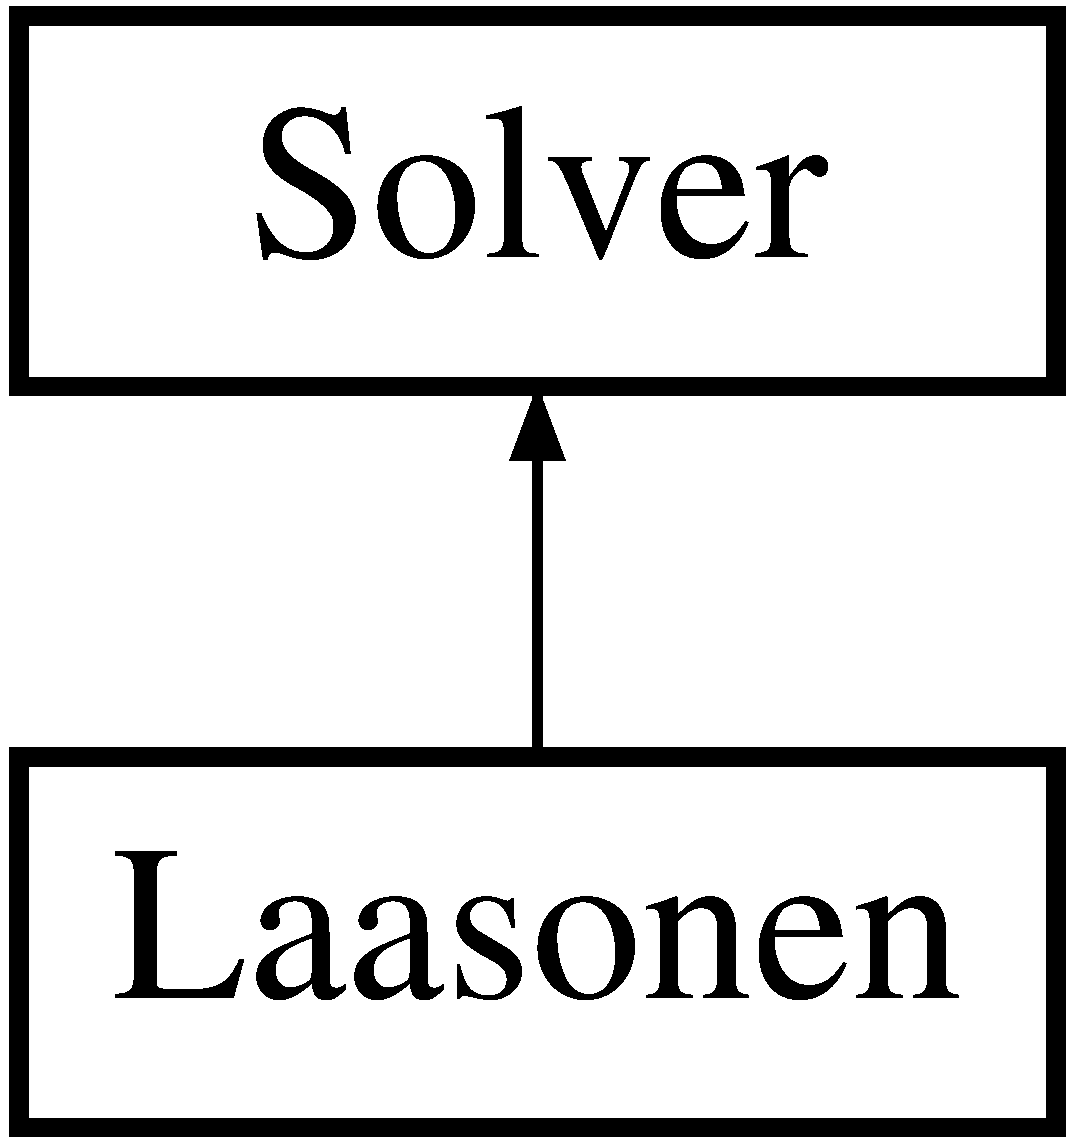
\includegraphics[height=2.000000cm]{classLaasonen}
\end{center}
\end{figure}
\subsection*{Public Member Functions}
\begin{DoxyCompactItemize}
\item 
\mbox{\hyperlink{classLaasonen_a947e0e719ea5ffc3c327df1efb021c8c}{Laasonen}} (double dx, double dt, double L, double T, double D, double Tsur, double Tin)
\item 
virtual \mbox{\hyperlink{classMatrix}{Matrix}} \mbox{\hyperlink{classLaasonen_ae16757353c84d22b3a444116a64a6375}{compute\+Solution}} ()
\end{DoxyCompactItemize}
\subsection*{Additional Inherited Members}


\subsection{Constructor \& Destructor Documentation}
\mbox{\Hypertarget{classLaasonen_a947e0e719ea5ffc3c327df1efb021c8c}\label{classLaasonen_a947e0e719ea5ffc3c327df1efb021c8c}} 
\index{Laasonen@{Laasonen}!Laasonen@{Laasonen}}
\index{Laasonen@{Laasonen}!Laasonen@{Laasonen}}
\subsubsection{\texorpdfstring{Laasonen()}{Laasonen()}}
{\footnotesize\ttfamily Laasonen\+::\+Laasonen (\begin{DoxyParamCaption}\item[{double}]{dx,  }\item[{double}]{dt,  }\item[{double}]{L,  }\item[{double}]{T,  }\item[{double}]{D,  }\item[{double}]{Tsur,  }\item[{double}]{Tin }\end{DoxyParamCaption})}

Construcs a solver of the problem using \mbox{\hyperlink{classLaasonen}{Laasonen}} method 
\begin{DoxyExceptions}{Exceptions}
{\em invalid\+\_\+argument} & (\char`\"{}dx should be positive\char`\"{}) \\
\hline
{\em invalid\+\_\+argument} & (\char`\"{}dt should be positive\char`\"{}) \\
\hline
{\em invalid\+\_\+argument} & (\char`\"{}\+L should be positive\char`\"{}) \\
\hline
{\em invalid\+\_\+argument} & (\char`\"{}\+T should be positive\char`\"{}) \\
\hline
{\em invalid\+\_\+argument} & (\char`\"{}\+L should be equal or larger than dx\char`\"{}) \\
\hline
{\em invalid\+\_\+argument} & (\char`\"{}\+T should be equal or larger than dt\char`\"{}) \\
\hline
\end{DoxyExceptions}

\begin{DoxyParams}{Parameters}
{\em dx} & double. distance between two space steps \\
\hline
{\em dt} & double. time between two time steps \\
\hline
{\em L} & double. width of the 1D material to consider \\
\hline
{\em T} & double. Total time of the considerated problem \\
\hline
{\em D} & double. Diffusion coefficient of the material \\
\hline
{\em Tsur} & double. The temperature that will be applied on the boundaries of the material \\
\hline
{\em Tin} & double. The initial temperature of the material \\
\hline
\end{DoxyParams}


\subsection{Member Function Documentation}
\mbox{\Hypertarget{classLaasonen_ae16757353c84d22b3a444116a64a6375}\label{classLaasonen_ae16757353c84d22b3a444116a64a6375}} 
\index{Laasonen@{Laasonen}!compute\+Solution@{compute\+Solution}}
\index{compute\+Solution@{compute\+Solution}!Laasonen@{Laasonen}}
\subsubsection{\texorpdfstring{compute\+Solution()}{computeSolution()}}
{\footnotesize\ttfamily \mbox{\hyperlink{classMatrix}{Matrix}} Laasonen\+::compute\+Solution (\begin{DoxyParamCaption}{ }\end{DoxyParamCaption})\hspace{0.3cm}{\ttfamily [virtual]}}

Compute the solution and return it. This method is the \mbox{\hyperlink{classLaasonen}{Laasonen}} method applied to the heat diffusion equation problem \begin{DoxyReturn}{Returns}
\mbox{\hyperlink{classMatrix}{Matrix}}. The computed matrix, can also be accesed through \mbox{\hyperlink{classSolver_aafe88ce4130c001052e5d93c1681f90f}{get\+Computed\+Solution()}} 
\end{DoxyReturn}
\begin{DoxySeeAlso}{See also}
\mbox{\hyperlink{classSolver_aafe88ce4130c001052e5d93c1681f90f}{get\+Computed\+Solution()}} 
\end{DoxySeeAlso}


Implements \mbox{\hyperlink{classSolver_a0f4ecfaed825407019995b5176e25748}{Solver}}.



The documentation for this class was generated from the following files\+:\begin{DoxyCompactItemize}
\item 
Laasonen.\+h\item 
Laasonen.\+cpp\end{DoxyCompactItemize}

\hypertarget{classMatrix}{}\section{Matrix Class Reference}
\label{classMatrix}\index{Matrix@{Matrix}}


{\ttfamily \#include $<$matrix.\+h$>$}

Inheritance diagram for Matrix\+:\begin{figure}[H]
\begin{center}
\leavevmode
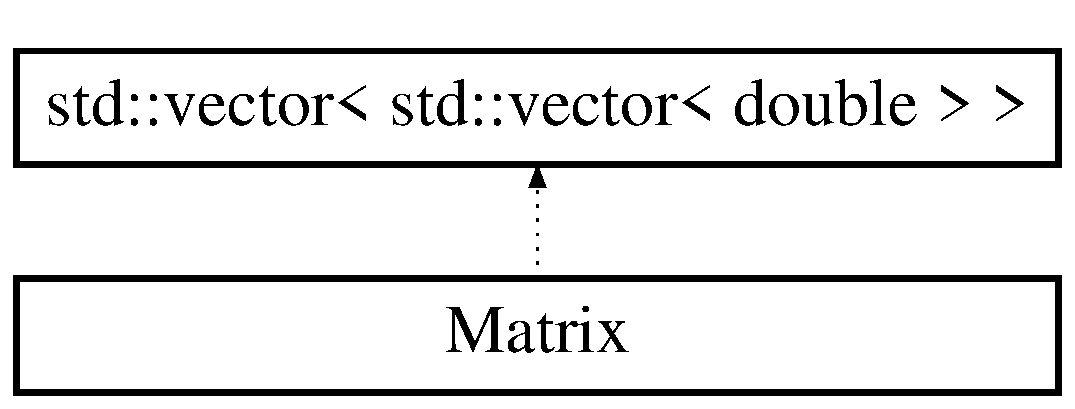
\includegraphics[height=2.000000cm]{classMatrix}
\end{center}
\end{figure}
\subsection*{Public Member Functions}
\begin{DoxyCompactItemize}
\item 
\mbox{\hyperlink{classMatrix_a2dba13c45127354c9f75ef576f49269b}{Matrix}} ()
\item 
\mbox{\hyperlink{classMatrix_a135a15de1126d735bb95fcc839d739d7}{Matrix}} (int Nrows, int Ncols)
\item 
\mbox{\hyperlink{classMatrix_a765f4dcb51b6829311cc3e7576388423}{Matrix}} (const \mbox{\hyperlink{classMatrix}{Matrix}} \&m)
\item 
int \mbox{\hyperlink{classMatrix_a711f84a1c62832d9d197d78c9855a276}{get\+Nrows}} () const
\item 
int \mbox{\hyperlink{classMatrix_ae0a5f2154953b8d129a90b04f91d9079}{get\+Ncols}} () const
\item 
\mbox{\hyperlink{classMatrix}{Matrix}} \& \mbox{\hyperlink{classMatrix_aea5a06385f646eb4a63929fae6fa3e14}{operator=}} (const \mbox{\hyperlink{classMatrix}{Matrix}} \&m)
\item 
bool \mbox{\hyperlink{classMatrix_a35097c20bcb1495b57d452db0d7b1f53}{operator==}} (const \mbox{\hyperlink{classMatrix}{Matrix}} \&m) const
\item 
double \mbox{\hyperlink{classMatrix_af4d468252f3ecbbcaa5726c76e332b4c}{one\+\_\+norm}} () const
\item 
double \mbox{\hyperlink{classMatrix_aac496af05ec7aa26afc2b9c6d0ab8b66}{two\+\_\+norm}} () const
\item 
double \mbox{\hyperlink{classMatrix_a43066c7fe6418aad40170b85415063e8}{uniform\+\_\+norm}} () const
\item 
\mbox{\hyperlink{classMatrix}{Matrix}} \mbox{\hyperlink{classMatrix_aaa40c78e6b3bb5bbf572d35612dbf6a7}{operator$\ast$}} (const \mbox{\hyperlink{classMatrix}{Matrix}} \&a) const
\item 
\mbox{\hyperlink{classMatrix}{Matrix}} \mbox{\hyperlink{classMatrix_a5f08ceb21dd13e2afa6c68afc73db1d3}{operator-\/}} (const \mbox{\hyperlink{classMatrix}{Matrix}} \&a) const
\item 
\mbox{\hyperlink{classVector}{Vector}} \mbox{\hyperlink{classMatrix_a843eebe2b6bd9d8091be600f685252cb}{operator$\ast$}} (const \mbox{\hyperlink{classVector}{Vector}} \&v) const
\item 
\mbox{\hyperlink{classMatrix}{Matrix}} \mbox{\hyperlink{classMatrix_a759661b75b9681f3a89ff75e27933b3a}{transpose}} () const
\end{DoxyCompactItemize}
\subsection*{Friends}
\begin{DoxyCompactItemize}
\item 
std\+::istream \& \mbox{\hyperlink{classMatrix_a3d6c1dcfc038804f4c08687f4f37f48b}{operator$>$$>$}} (std\+::istream \&is, \mbox{\hyperlink{classMatrix}{Matrix}} \&m)
\item 
std\+::ostream \& \mbox{\hyperlink{classMatrix_a060711074cb5bcaf4e75498bc040c4b7}{operator$<$$<$}} (std\+::ostream \&os, const \mbox{\hyperlink{classMatrix}{Matrix}} \&m)
\item 
std\+::ifstream \& \mbox{\hyperlink{classMatrix_aa5699a0bdf0ee014f083ff8a76629d21}{operator$>$$>$}} (std\+::ifstream \&ifs, \mbox{\hyperlink{classMatrix}{Matrix}} \&m)
\item 
std\+::ofstream \& \mbox{\hyperlink{classMatrix_aa574249d63b390cf1108d6e82047ef61}{operator$<$$<$}} (std\+::ofstream \&ofs, const \mbox{\hyperlink{classMatrix}{Matrix}} \&m)
\end{DoxyCompactItemize}


\subsection{Detailed Description}
A matrix class for data storage of a 2D array of doubles ~\newline
 The implementation is derived from the standard container vector std\+::vector ~\newline
 We use private inheritance to base our vector upon the library version whilst  usto expose only those base class functions we wish to use -\/ in this  the array access operator \mbox{[}\mbox{]}

The \mbox{\hyperlink{classMatrix}{Matrix}} class provides\+: ~\newline
-\/basic constructors for creating a matrix object from other matrix object,  by creating empty matrix of a given size, ~\newline
-\/input and oput operation via $>$$>$ and $<$$<$ operators using keyboard or file ~\newline
-\/basic operations like access via \mbox{[}\mbox{]} operator, assignment and comparision 

\subsection{Constructor \& Destructor Documentation}
\mbox{\Hypertarget{classMatrix_a2dba13c45127354c9f75ef576f49269b}\label{classMatrix_a2dba13c45127354c9f75ef576f49269b}} 
\index{Matrix@{Matrix}!Matrix@{Matrix}}
\index{Matrix@{Matrix}!Matrix@{Matrix}}
\subsubsection{\texorpdfstring{Matrix()}{Matrix()}\hspace{0.1cm}{\footnotesize\ttfamily [1/3]}}
{\footnotesize\ttfamily Matrix\+::\+Matrix (\begin{DoxyParamCaption}{ }\end{DoxyParamCaption})}

Default constructor. Intialize an empty \mbox{\hyperlink{classMatrix}{Matrix}} object \begin{DoxySeeAlso}{See also}
\mbox{\hyperlink{classMatrix_a135a15de1126d735bb95fcc839d739d7}{Matrix(int Nrows, int Ncols)}} 

\mbox{\hyperlink{classMatrix_a765f4dcb51b6829311cc3e7576388423}{Matrix(const Matrix\& m)}} 
\end{DoxySeeAlso}
\mbox{\Hypertarget{classMatrix_a135a15de1126d735bb95fcc839d739d7}\label{classMatrix_a135a15de1126d735bb95fcc839d739d7}} 
\index{Matrix@{Matrix}!Matrix@{Matrix}}
\index{Matrix@{Matrix}!Matrix@{Matrix}}
\subsubsection{\texorpdfstring{Matrix()}{Matrix()}\hspace{0.1cm}{\footnotesize\ttfamily [2/3]}}
{\footnotesize\ttfamily Matrix\+::\+Matrix (\begin{DoxyParamCaption}\item[{int}]{Nrows,  }\item[{int}]{Ncols }\end{DoxyParamCaption})}

Alternate constructor. build a matrix Nrows by Ncols \begin{DoxySeeAlso}{See also}
\mbox{\hyperlink{classMatrix_a2dba13c45127354c9f75ef576f49269b}{Matrix()}} 

\mbox{\hyperlink{classMatrix_a765f4dcb51b6829311cc3e7576388423}{Matrix(const Matrix\& m)}} 
\end{DoxySeeAlso}

\begin{DoxyExceptions}{Exceptions}
{\em invalid\+\_\+argument} & (\char`\"{}matrix size negative or zero\char`\"{}) \\
\hline
\end{DoxyExceptions}

\begin{DoxyParams}{Parameters}
{\em Nrows} & int. number of rows in matrix \\
\hline
{\em Ncols} & int. number of columns in matrix \\
\hline
\end{DoxyParams}
\mbox{\Hypertarget{classMatrix_a765f4dcb51b6829311cc3e7576388423}\label{classMatrix_a765f4dcb51b6829311cc3e7576388423}} 
\index{Matrix@{Matrix}!Matrix@{Matrix}}
\index{Matrix@{Matrix}!Matrix@{Matrix}}
\subsubsection{\texorpdfstring{Matrix()}{Matrix()}\hspace{0.1cm}{\footnotesize\ttfamily [3/3]}}
{\footnotesize\ttfamily Matrix\+::\+Matrix (\begin{DoxyParamCaption}\item[{const \mbox{\hyperlink{classMatrix}{Matrix}} \&}]{m }\end{DoxyParamCaption})}

Copy constructor. build a matrix from another matrix \begin{DoxySeeAlso}{See also}
\mbox{\hyperlink{classMatrix_a2dba13c45127354c9f75ef576f49269b}{Matrix()}} 

\mbox{\hyperlink{classMatrix_a135a15de1126d735bb95fcc839d739d7}{Matrix(int Nrows, int Ncols)}} 
\end{DoxySeeAlso}

\begin{DoxyParams}{Parameters}
{\em m} & \mbox{\hyperlink{classMatrix}{Matrix}}\&. matrix to copy from \\
\hline
\end{DoxyParams}


\subsection{Member Function Documentation}
\mbox{\Hypertarget{classMatrix_ae0a5f2154953b8d129a90b04f91d9079}\label{classMatrix_ae0a5f2154953b8d129a90b04f91d9079}} 
\index{Matrix@{Matrix}!get\+Ncols@{get\+Ncols}}
\index{get\+Ncols@{get\+Ncols}!Matrix@{Matrix}}
\subsubsection{\texorpdfstring{get\+Ncols()}{getNcols()}}
{\footnotesize\ttfamily int Matrix\+::get\+Ncols (\begin{DoxyParamCaption}{ }\end{DoxyParamCaption}) const}

Normal public get method. get the number of columns \begin{DoxySeeAlso}{See also}
int \mbox{\hyperlink{classMatrix_a711f84a1c62832d9d197d78c9855a276}{get\+Nrows()const}} 
\end{DoxySeeAlso}
\begin{DoxyReturn}{Returns}
int. number of columns in matrix 
\end{DoxyReturn}
\mbox{\Hypertarget{classMatrix_a711f84a1c62832d9d197d78c9855a276}\label{classMatrix_a711f84a1c62832d9d197d78c9855a276}} 
\index{Matrix@{Matrix}!get\+Nrows@{get\+Nrows}}
\index{get\+Nrows@{get\+Nrows}!Matrix@{Matrix}}
\subsubsection{\texorpdfstring{get\+Nrows()}{getNrows()}}
{\footnotesize\ttfamily int Matrix\+::get\+Nrows (\begin{DoxyParamCaption}{ }\end{DoxyParamCaption}) const}

Normal public get method. get the number of rows \begin{DoxySeeAlso}{See also}
int \mbox{\hyperlink{classMatrix_ae0a5f2154953b8d129a90b04f91d9079}{get\+Ncols()const}} 
\end{DoxySeeAlso}
\begin{DoxyReturn}{Returns}
int. number of rows in matrix 
\end{DoxyReturn}
\mbox{\Hypertarget{classMatrix_af4d468252f3ecbbcaa5726c76e332b4c}\label{classMatrix_af4d468252f3ecbbcaa5726c76e332b4c}} 
\index{Matrix@{Matrix}!one\+\_\+norm@{one\+\_\+norm}}
\index{one\+\_\+norm@{one\+\_\+norm}!Matrix@{Matrix}}
\subsubsection{\texorpdfstring{one\+\_\+norm()}{one\_norm()}}
{\footnotesize\ttfamily double Matrix\+::one\+\_\+norm (\begin{DoxyParamCaption}{ }\end{DoxyParamCaption}) const}

Normal public method that returns a double. It returns L1 norm of matrix \begin{DoxySeeAlso}{See also}
\mbox{\hyperlink{classMatrix_aac496af05ec7aa26afc2b9c6d0ab8b66}{two\+\_\+norm()const}} 

\mbox{\hyperlink{classMatrix_a43066c7fe6418aad40170b85415063e8}{uniform\+\_\+norm()const}} 
\end{DoxySeeAlso}
\begin{DoxyReturn}{Returns}
double. matrix L1 norm 
\end{DoxyReturn}
\mbox{\Hypertarget{classMatrix_aaa40c78e6b3bb5bbf572d35612dbf6a7}\label{classMatrix_aaa40c78e6b3bb5bbf572d35612dbf6a7}} 
\index{Matrix@{Matrix}!operator$\ast$@{operator$\ast$}}
\index{operator$\ast$@{operator$\ast$}!Matrix@{Matrix}}
\subsubsection{\texorpdfstring{operator$\ast$()}{operator*()}\hspace{0.1cm}{\footnotesize\ttfamily [1/2]}}
{\footnotesize\ttfamily \mbox{\hyperlink{classMatrix}{Matrix}} Matrix\+::operator$\ast$ (\begin{DoxyParamCaption}\item[{const \mbox{\hyperlink{classMatrix}{Matrix}} \&}]{a }\end{DoxyParamCaption}) const}

Overloaded $\ast$operator that returns a \mbox{\hyperlink{classMatrix}{Matrix}}. It Performs matrix by matrix multiplication. \begin{DoxySeeAlso}{See also}
\mbox{\hyperlink{classMatrix_aaa40c78e6b3bb5bbf572d35612dbf6a7}{operator$\ast$(const Matrix \& a) const}} 
\end{DoxySeeAlso}

\begin{DoxyExceptions}{Exceptions}
{\em out\+\_\+of\+\_\+range} & (\char`\"{}\+Matrix access error\char`\"{}) One or more of the matrix have a zero size \\
\hline
{\em std\+::out\+\_\+of\+\_\+range} & (\char`\"{}uncompatible matrix sizes\char`\"{}) Number of columns in first matrix do not match number of columns in second matrix \\
\hline
\end{DoxyExceptions}
\begin{DoxyReturn}{Returns}
\mbox{\hyperlink{classMatrix}{Matrix}}. matrix-\/matrix product 
\end{DoxyReturn}

\begin{DoxyParams}{Parameters}
{\em a} & \mbox{\hyperlink{classMatrix}{Matrix}}. matrix to multiply by \\
\hline
\end{DoxyParams}
\mbox{\Hypertarget{classMatrix_a843eebe2b6bd9d8091be600f685252cb}\label{classMatrix_a843eebe2b6bd9d8091be600f685252cb}} 
\index{Matrix@{Matrix}!operator$\ast$@{operator$\ast$}}
\index{operator$\ast$@{operator$\ast$}!Matrix@{Matrix}}
\subsubsection{\texorpdfstring{operator$\ast$()}{operator*()}\hspace{0.1cm}{\footnotesize\ttfamily [2/2]}}
{\footnotesize\ttfamily \mbox{\hyperlink{classVector}{Vector}} Matrix\+::operator$\ast$ (\begin{DoxyParamCaption}\item[{const \mbox{\hyperlink{classVector}{Vector}} \&}]{v }\end{DoxyParamCaption}) const}

Overloaded $\ast$operator that returns a \mbox{\hyperlink{classVector}{Vector}}. It Performs matrix by vector multiplication. \begin{DoxySeeAlso}{See also}
\mbox{\hyperlink{classMatrix_aaa40c78e6b3bb5bbf572d35612dbf6a7}{operator$\ast$(const Matrix \& a)const}} 
\end{DoxySeeAlso}

\begin{DoxyExceptions}{Exceptions}
{\em std\+::out\+\_\+of\+\_\+range} & (\char`\"{}\+Matrix access error\char`\"{}) matrix has a zero size \\
\hline
{\em std\+::out\+\_\+of\+\_\+range} & (\char`\"{}\+Vector access error\char`\"{}) vector has a zero size \\
\hline
{\em std\+::out\+\_\+of\+\_\+range} & (\char`\"{}uncompatible matrix-\/vector sizes\char`\"{}) Number of columns in matrix do not match the vector size \\
\hline
\end{DoxyExceptions}
\begin{DoxyReturn}{Returns}
\mbox{\hyperlink{classVector}{Vector}}. matrix-\/vector product 
\end{DoxyReturn}

\begin{DoxyParams}{Parameters}
{\em v} & \mbox{\hyperlink{classVector}{Vector}}. \mbox{\hyperlink{classVector}{Vector}} to multiply by \\
\hline
\end{DoxyParams}
\mbox{\Hypertarget{classMatrix_a5f08ceb21dd13e2afa6c68afc73db1d3}\label{classMatrix_a5f08ceb21dd13e2afa6c68afc73db1d3}} 
\index{Matrix@{Matrix}!operator-\/@{operator-\/}}
\index{operator-\/@{operator-\/}!Matrix@{Matrix}}
\subsubsection{\texorpdfstring{operator-\/()}{operator-()}}
{\footnotesize\ttfamily \mbox{\hyperlink{classMatrix}{Matrix}} Matrix\+::operator-\/ (\begin{DoxyParamCaption}\item[{const \mbox{\hyperlink{classMatrix}{Matrix}} \&}]{a }\end{DoxyParamCaption}) const}

Overloaded -\/operator that returns a \mbox{\hyperlink{classMatrix}{Matrix}}. It Performs matrix by matrix substraction. \begin{DoxySeeAlso}{See also}
\mbox{\hyperlink{classMatrix_a5f08ceb21dd13e2afa6c68afc73db1d3}{operator-\/(const Matrix \& a) const}} 
\end{DoxySeeAlso}

\begin{DoxyExceptions}{Exceptions}
{\em out\+\_\+of\+\_\+range} & (\char`\"{}\+Matrix access error\char`\"{}) One or more of the matrix have a zero size \\
\hline
{\em std\+::out\+\_\+of\+\_\+range} & (\char`\"{}uncompatible matrix sizes\char`\"{}) Number of columns/rows in first matrix do not match number of columns or/and rows in second matrix \\
\hline
\end{DoxyExceptions}
\begin{DoxyReturn}{Returns}
\mbox{\hyperlink{classMatrix}{Matrix}}. matrix-\/matrix product 
\end{DoxyReturn}

\begin{DoxyParams}{Parameters}
{\em a} & \mbox{\hyperlink{classMatrix}{Matrix}}. matrix to multiply by \\
\hline
\end{DoxyParams}
\mbox{\Hypertarget{classMatrix_aea5a06385f646eb4a63929fae6fa3e14}\label{classMatrix_aea5a06385f646eb4a63929fae6fa3e14}} 
\index{Matrix@{Matrix}!operator=@{operator=}}
\index{operator=@{operator=}!Matrix@{Matrix}}
\subsubsection{\texorpdfstring{operator=()}{operator=()}}
{\footnotesize\ttfamily \mbox{\hyperlink{classMatrix}{Matrix}} \& Matrix\+::operator= (\begin{DoxyParamCaption}\item[{const \mbox{\hyperlink{classMatrix}{Matrix}} \&}]{m }\end{DoxyParamCaption})}

Overloaded assignment operator \begin{DoxySeeAlso}{See also}
\mbox{\hyperlink{classMatrix_a35097c20bcb1495b57d452db0d7b1f53}{operator==(const Matrix\& m)const}} 
\end{DoxySeeAlso}
\begin{DoxyReturn}{Returns}
\mbox{\hyperlink{classMatrix}{Matrix}}\&. the matrix on the left of the assignment 
\end{DoxyReturn}

\begin{DoxyParams}{Parameters}
{\em m} & \mbox{\hyperlink{classMatrix}{Matrix}}\&. \mbox{\hyperlink{classMatrix}{Matrix}} to assign from \\
\hline
\end{DoxyParams}
\mbox{\Hypertarget{classMatrix_a35097c20bcb1495b57d452db0d7b1f53}\label{classMatrix_a35097c20bcb1495b57d452db0d7b1f53}} 
\index{Matrix@{Matrix}!operator==@{operator==}}
\index{operator==@{operator==}!Matrix@{Matrix}}
\subsubsection{\texorpdfstring{operator==()}{operator==()}}
{\footnotesize\ttfamily bool Matrix\+::operator== (\begin{DoxyParamCaption}\item[{const \mbox{\hyperlink{classMatrix}{Matrix}} \&}]{m }\end{DoxyParamCaption}) const}

Overloaded comparison operator returns true or false depending on whether the matrices are the same or not \begin{DoxySeeAlso}{See also}
\mbox{\hyperlink{classMatrix_aea5a06385f646eb4a63929fae6fa3e14}{operator=(const Matrix\& m)}} 
\end{DoxySeeAlso}
\begin{DoxyReturn}{Returns}
bool. true or false 
\end{DoxyReturn}

\begin{DoxyParams}{Parameters}
{\em m} & \mbox{\hyperlink{classMatrix}{Matrix}}\&. \mbox{\hyperlink{classMatrix}{Matrix}} to compare to \\
\hline
\end{DoxyParams}
\mbox{\Hypertarget{classMatrix_a759661b75b9681f3a89ff75e27933b3a}\label{classMatrix_a759661b75b9681f3a89ff75e27933b3a}} 
\index{Matrix@{Matrix}!transpose@{transpose}}
\index{transpose@{transpose}!Matrix@{Matrix}}
\subsubsection{\texorpdfstring{transpose()}{transpose()}}
{\footnotesize\ttfamily \mbox{\hyperlink{classMatrix}{Matrix}} Matrix\+::transpose (\begin{DoxyParamCaption}{ }\end{DoxyParamCaption}) const}

public method that returns the transpose of the matrix. It returns the transpose of matrix \begin{DoxyReturn}{Returns}
\mbox{\hyperlink{classMatrix}{Matrix}}. matrix transpose 
\end{DoxyReturn}
\mbox{\Hypertarget{classMatrix_aac496af05ec7aa26afc2b9c6d0ab8b66}\label{classMatrix_aac496af05ec7aa26afc2b9c6d0ab8b66}} 
\index{Matrix@{Matrix}!two\+\_\+norm@{two\+\_\+norm}}
\index{two\+\_\+norm@{two\+\_\+norm}!Matrix@{Matrix}}
\subsubsection{\texorpdfstring{two\+\_\+norm()}{two\_norm()}}
{\footnotesize\ttfamily double Matrix\+::two\+\_\+norm (\begin{DoxyParamCaption}{ }\end{DoxyParamCaption}) const}

Normal public method that returns a double. It returns L2 norm of matrix \begin{DoxySeeAlso}{See also}
\mbox{\hyperlink{classMatrix_af4d468252f3ecbbcaa5726c76e332b4c}{one\+\_\+norm()const}} 

\mbox{\hyperlink{classMatrix_a43066c7fe6418aad40170b85415063e8}{uniform\+\_\+norm()const}} 
\end{DoxySeeAlso}
\begin{DoxyReturn}{Returns}
double. matrix L2 norm 
\end{DoxyReturn}
\mbox{\Hypertarget{classMatrix_a43066c7fe6418aad40170b85415063e8}\label{classMatrix_a43066c7fe6418aad40170b85415063e8}} 
\index{Matrix@{Matrix}!uniform\+\_\+norm@{uniform\+\_\+norm}}
\index{uniform\+\_\+norm@{uniform\+\_\+norm}!Matrix@{Matrix}}
\subsubsection{\texorpdfstring{uniform\+\_\+norm()}{uniform\_norm()}}
{\footnotesize\ttfamily double Matrix\+::uniform\+\_\+norm (\begin{DoxyParamCaption}{ }\end{DoxyParamCaption}) const}

Normal public method that returns a double. It returns L\+\_\+max norm of matrix \begin{DoxySeeAlso}{See also}
\mbox{\hyperlink{classMatrix_af4d468252f3ecbbcaa5726c76e332b4c}{one\+\_\+norm()const}} 

\mbox{\hyperlink{classMatrix_aac496af05ec7aa26afc2b9c6d0ab8b66}{two\+\_\+norm()const}} 
\end{DoxySeeAlso}
\begin{DoxyReturn}{Returns}
double. matrix L\+\_\+max norm 
\end{DoxyReturn}


\subsection{Friends And Related Function Documentation}
\mbox{\Hypertarget{classMatrix_a060711074cb5bcaf4e75498bc040c4b7}\label{classMatrix_a060711074cb5bcaf4e75498bc040c4b7}} 
\index{Matrix@{Matrix}!operator$<$$<$@{operator$<$$<$}}
\index{operator$<$$<$@{operator$<$$<$}!Matrix@{Matrix}}
\subsubsection{\texorpdfstring{operator$<$$<$}{operator<<}\hspace{0.1cm}{\footnotesize\ttfamily [1/2]}}
{\footnotesize\ttfamily std\+::ostream\& operator$<$$<$ (\begin{DoxyParamCaption}\item[{std\+::ostream \&}]{os,  }\item[{const \mbox{\hyperlink{classMatrix}{Matrix}} \&}]{m }\end{DoxyParamCaption})\hspace{0.3cm}{\ttfamily [friend]}}

Overloaded ostream $<$$<$ operator. Display output if matrix has size user will be asked to input only matrix values if matrix was not initialized user can choose matrix size and input it values \begin{DoxySeeAlso}{See also}
\mbox{\hyperlink{classMatrix_aa5699a0bdf0ee014f083ff8a76629d21}{operator$>$$>$(std\+::ifstream\& ifs, Matrix\& m)}} 

\mbox{\hyperlink{classMatrix_a3d6c1dcfc038804f4c08687f4f37f48b}{operator$>$$>$(std\+::istream\& is, Matrix\& m)}} 

\mbox{\hyperlink{classMatrix_a060711074cb5bcaf4e75498bc040c4b7}{operator$<$$<$(std\+::ostream\& os, const Matrix\& m)}} 
\end{DoxySeeAlso}
\begin{DoxyReturn}{Returns}
std\+::ostream\&. The ostream object 
\end{DoxyReturn}

\begin{DoxyParams}{Parameters}
{\em os} & Display output stream \\
\hline
{\em m} & \mbox{\hyperlink{classMatrix}{Matrix}} to read from \\
\hline
\end{DoxyParams}
\mbox{\Hypertarget{classMatrix_aa574249d63b390cf1108d6e82047ef61}\label{classMatrix_aa574249d63b390cf1108d6e82047ef61}} 
\index{Matrix@{Matrix}!operator$<$$<$@{operator$<$$<$}}
\index{operator$<$$<$@{operator$<$$<$}!Matrix@{Matrix}}
\subsubsection{\texorpdfstring{operator$<$$<$}{operator<<}\hspace{0.1cm}{\footnotesize\ttfamily [2/2]}}
{\footnotesize\ttfamily std\+::ofstream\& operator$<$$<$ (\begin{DoxyParamCaption}\item[{std\+::ofstream \&}]{ofs,  }\item[{const \mbox{\hyperlink{classMatrix}{Matrix}} \&}]{m }\end{DoxyParamCaption})\hspace{0.3cm}{\ttfamily [friend]}}

Overloaded ofstream $<$$<$ operator. File output the file output operator is compatible with file input operator, ie. everything written can be read later. \begin{DoxySeeAlso}{See also}
\mbox{\hyperlink{classMatrix_aa5699a0bdf0ee014f083ff8a76629d21}{operator$>$$>$(std\+::ifstream\& ifs, Matrix\& m)}} 

\mbox{\hyperlink{classMatrix_aa574249d63b390cf1108d6e82047ef61}{operator$<$$<$(std\+::ofstream\& ofs, const Matrix\& m)}} 

\mbox{\hyperlink{classMatrix_a3d6c1dcfc038804f4c08687f4f37f48b}{operator$>$$>$(std\+::istream\& is, Matrix\& m)}} 
\end{DoxySeeAlso}

\begin{DoxyExceptions}{Exceptions}
{\em std\+::invalid\+\_\+argument} & (\char`\"{}file read error -\/ negative matrix size\char`\"{}); \\
\hline
\end{DoxyExceptions}
\begin{DoxyReturn}{Returns}
std\+::ofstream\&. The ofstream object 
\end{DoxyReturn}

\begin{DoxyParams}{Parameters}
{\em m} & \mbox{\hyperlink{classMatrix}{Matrix}} to read from \\
\hline
\end{DoxyParams}
\mbox{\Hypertarget{classMatrix_a3d6c1dcfc038804f4c08687f4f37f48b}\label{classMatrix_a3d6c1dcfc038804f4c08687f4f37f48b}} 
\index{Matrix@{Matrix}!operator$>$$>$@{operator$>$$>$}}
\index{operator$>$$>$@{operator$>$$>$}!Matrix@{Matrix}}
\subsubsection{\texorpdfstring{operator$>$$>$}{operator>>}\hspace{0.1cm}{\footnotesize\ttfamily [1/2]}}
{\footnotesize\ttfamily std\+::istream\& operator$>$$>$ (\begin{DoxyParamCaption}\item[{std\+::istream \&}]{is,  }\item[{\mbox{\hyperlink{classMatrix}{Matrix}} \&}]{m }\end{DoxyParamCaption})\hspace{0.3cm}{\ttfamily [friend]}}

Overloaded istream $>$$>$ operator. Keyboard input if matrix has size user will be asked to input only matrix values if matrix was not initialized user can choose matrix size and input it values \begin{DoxySeeAlso}{See also}
\mbox{\hyperlink{classMatrix_aa574249d63b390cf1108d6e82047ef61}{operator$<$$<$(std\+::ofstream\& ofs, const Matrix\& m)}} 

\mbox{\hyperlink{classMatrix_a3d6c1dcfc038804f4c08687f4f37f48b}{operator$>$$>$(std\+::istream\& is, Matrix\& m)}} 

\mbox{\hyperlink{classMatrix_a060711074cb5bcaf4e75498bc040c4b7}{operator$<$$<$(std\+::ostream\& os, const Matrix\& m)}} 
\end{DoxySeeAlso}

\begin{DoxyExceptions}{Exceptions}
{\em std\+::invalid\+\_\+argument} & (\char`\"{}read error -\/ negative matrix size\char`\"{}); \\
\hline
\end{DoxyExceptions}
\begin{DoxyReturn}{Returns}
std\+::istream\&. The istream object 
\end{DoxyReturn}

\begin{DoxyParams}{Parameters}
{\em is} & Keyboard input stream \\
\hline
{\em m} & \mbox{\hyperlink{classMatrix}{Matrix}} to write into \\
\hline
\end{DoxyParams}
\mbox{\Hypertarget{classMatrix_aa5699a0bdf0ee014f083ff8a76629d21}\label{classMatrix_aa5699a0bdf0ee014f083ff8a76629d21}} 
\index{Matrix@{Matrix}!operator$>$$>$@{operator$>$$>$}}
\index{operator$>$$>$@{operator$>$$>$}!Matrix@{Matrix}}
\subsubsection{\texorpdfstring{operator$>$$>$}{operator>>}\hspace{0.1cm}{\footnotesize\ttfamily [2/2]}}
{\footnotesize\ttfamily std\+::ifstream\& operator$>$$>$ (\begin{DoxyParamCaption}\item[{std\+::ifstream \&}]{ifs,  }\item[{\mbox{\hyperlink{classMatrix}{Matrix}} \&}]{m }\end{DoxyParamCaption})\hspace{0.3cm}{\ttfamily [friend]}}

Overloaded ifstream $>$$>$ operator. File input the file output operator is compatible with file input operator, ie. everything written can be read later. \begin{DoxySeeAlso}{See also}
\mbox{\hyperlink{classMatrix_aa5699a0bdf0ee014f083ff8a76629d21}{operator$>$$>$(std\+::ifstream\& ifs, Matrix\& m)}} 

\mbox{\hyperlink{classMatrix_aa574249d63b390cf1108d6e82047ef61}{operator$<$$<$(std\+::ofstream\& ofs, const Matrix\& m)}} 

\mbox{\hyperlink{classMatrix_a060711074cb5bcaf4e75498bc040c4b7}{operator$<$$<$(std\+::ostream\& os, const Matrix\& m)}} 
\end{DoxySeeAlso}
\begin{DoxyReturn}{Returns}
std\+::ifstream\&. The ifstream object 
\end{DoxyReturn}

\begin{DoxyParams}{Parameters}
{\em ifs} & Input file stream with opened matrix file \\
\hline
{\em m} & \mbox{\hyperlink{classMatrix}{Matrix}} to write into \\
\hline
\end{DoxyParams}


The documentation for this class was generated from the following files\+:\begin{DoxyCompactItemize}
\item 
matrix.\+h\item 
matrix.\+cpp\end{DoxyCompactItemize}

\hypertarget{classRichardson}{}\section{Richardson Class Reference}
\label{classRichardson}\index{Richardson@{Richardson}}
Inheritance diagram for Richardson\+:\begin{figure}[H]
\begin{center}
\leavevmode
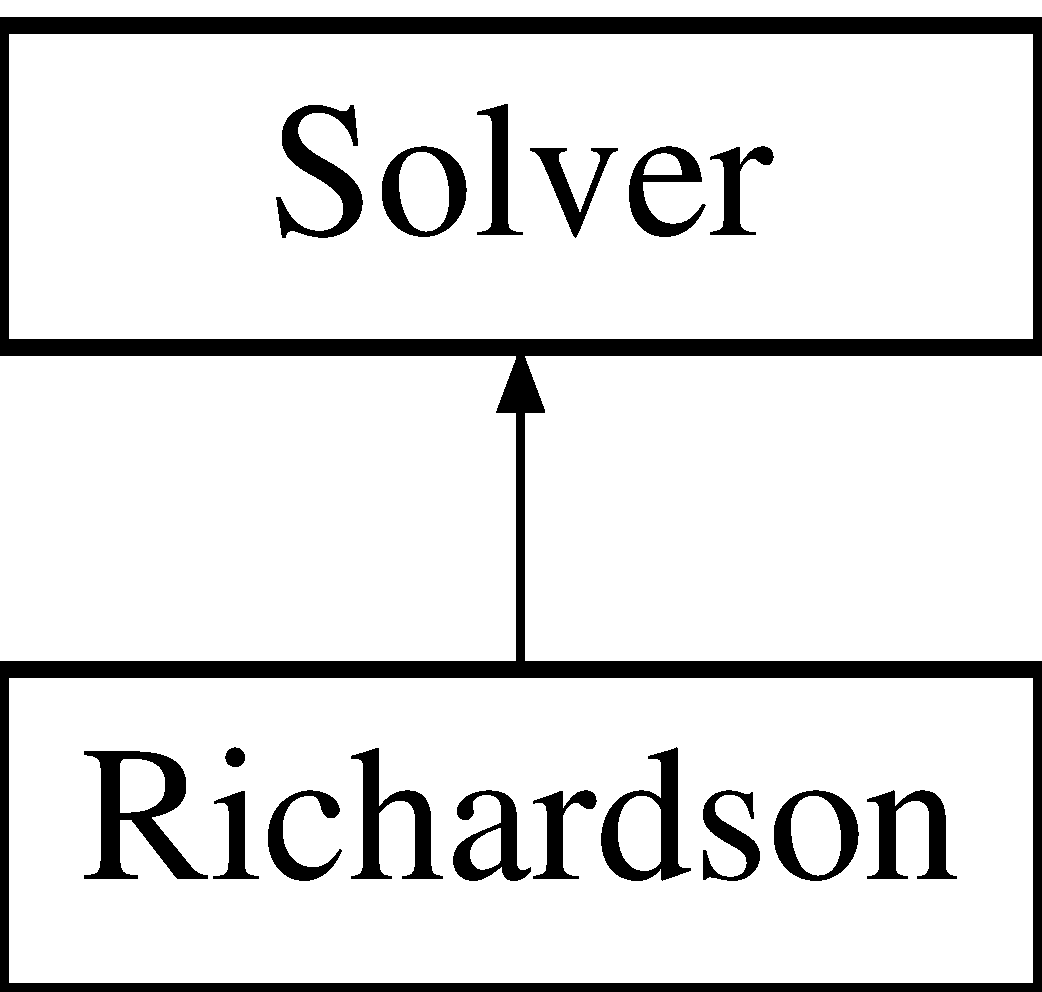
\includegraphics[height=2.000000cm]{classRichardson}
\end{center}
\end{figure}
\subsection*{Public Member Functions}
\begin{DoxyCompactItemize}
\item 
\mbox{\hyperlink{classRichardson_a43802f7613bfd6074da2c823a6bbbb2c}{Richardson}} (double dx, double dt, double L, double T, double D, double Tsur, double Tin)
\item 
virtual \mbox{\hyperlink{classMatrix}{Matrix}} \mbox{\hyperlink{classRichardson_a8d2471f20a6b433cf7ccf5a4817b14a3}{compute\+Solution}} ()
\end{DoxyCompactItemize}
\subsection*{Additional Inherited Members}


\subsection{Constructor \& Destructor Documentation}
\mbox{\Hypertarget{classRichardson_a43802f7613bfd6074da2c823a6bbbb2c}\label{classRichardson_a43802f7613bfd6074da2c823a6bbbb2c}} 
\index{Richardson@{Richardson}!Richardson@{Richardson}}
\index{Richardson@{Richardson}!Richardson@{Richardson}}
\subsubsection{\texorpdfstring{Richardson()}{Richardson()}}
{\footnotesize\ttfamily Richardson\+::\+Richardson (\begin{DoxyParamCaption}\item[{double}]{dx,  }\item[{double}]{dt,  }\item[{double}]{L,  }\item[{double}]{T,  }\item[{double}]{D,  }\item[{double}]{Tsur,  }\item[{double}]{Tin }\end{DoxyParamCaption})}

Construcs a solver of the problem using \mbox{\hyperlink{classRichardson}{Richardson}} method 
\begin{DoxyParams}{Parameters}
{\em dx} & double. distance between two space steps \\
\hline
{\em dt} & double. time between two time steps \\
\hline
{\em L} & double. width of the 1D material to consider \\
\hline
{\em T} & double. Total time of the considerated problem \\
\hline
{\em D} & double. Diffusion coefficient of the material \\
\hline
{\em Tsur} & double. The temperature that will be applied on the boundaries of the material \\
\hline
{\em Tin} & double. The initial temperature of the material \\
\hline
\end{DoxyParams}


\subsection{Member Function Documentation}
\mbox{\Hypertarget{classRichardson_a8d2471f20a6b433cf7ccf5a4817b14a3}\label{classRichardson_a8d2471f20a6b433cf7ccf5a4817b14a3}} 
\index{Richardson@{Richardson}!compute\+Solution@{compute\+Solution}}
\index{compute\+Solution@{compute\+Solution}!Richardson@{Richardson}}
\subsubsection{\texorpdfstring{compute\+Solution()}{computeSolution()}}
{\footnotesize\ttfamily \mbox{\hyperlink{classMatrix}{Matrix}} Richardson\+::compute\+Solution (\begin{DoxyParamCaption}{ }\end{DoxyParamCaption})\hspace{0.3cm}{\ttfamily [virtual]}}

Compute the solution and return it. This method is the \mbox{\hyperlink{classRichardson}{Richardson}} method applied to the heat diffusion equation problem \begin{DoxyReturn}{Returns}
\mbox{\hyperlink{classMatrix}{Matrix}}. The computed matrix, can also be accesed through \mbox{\hyperlink{classSolver_aafe88ce4130c001052e5d93c1681f90f}{get\+Computed\+Solution()}} 
\end{DoxyReturn}
\begin{DoxySeeAlso}{See also}
\mbox{\hyperlink{classSolver_aafe88ce4130c001052e5d93c1681f90f}{get\+Computed\+Solution()}} 
\end{DoxySeeAlso}


Implements \mbox{\hyperlink{classSolver_a0f4ecfaed825407019995b5176e25748}{Solver}}.



The documentation for this class was generated from the following files\+:\begin{DoxyCompactItemize}
\item 
Richardson.\+h\item 
Richardson.\+cpp\end{DoxyCompactItemize}

\hypertarget{classSolver}{}\section{Solver Class Reference}
\label{classSolver}\index{Solver@{Solver}}
Inheritance diagram for Solver\+:\begin{figure}[H]
\begin{center}
\leavevmode
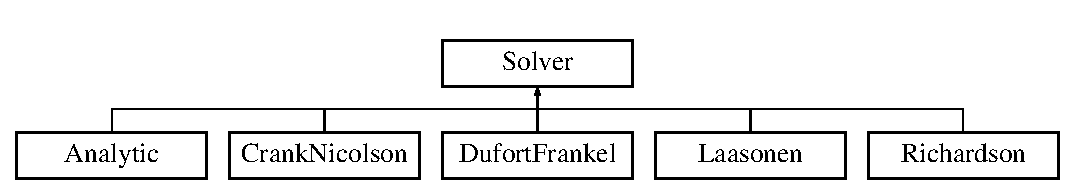
\includegraphics[height=2.000000cm]{classSolver}
\end{center}
\end{figure}
\subsection*{Public Member Functions}
\begin{DoxyCompactItemize}
\item 
\mbox{\hyperlink{classSolver_a3a1edb79e38781d40e5be114c7a549ba}{Solver}} (double dx, double dt, double L, double T, double D, double Tsur, double Tin)
\item 
\mbox{\hyperlink{classMatrix}{Matrix}} \mbox{\hyperlink{classSolver_aafe88ce4130c001052e5d93c1681f90f}{get\+Computed\+Solution}} ()
\item 
double \mbox{\hyperlink{classSolver_a560a332c3193d5709e1e5eb44bfaa322}{get\+DT}} ()
\item 
double \mbox{\hyperlink{classSolver_a6a05cda84ae4e3f3a187cf69f1407d81}{get\+DX}} ()
\item 
double \mbox{\hyperlink{classSolver_afb4f245f8c8109afb3301942d30b4544}{getL}} ()
\item 
double \mbox{\hyperlink{classSolver_a7a09182372f91099da1cba8b1527e4c7}{getT}} ()
\item 
double \mbox{\hyperlink{classSolver_a3b4da24979dd1c316c860749bbf6e3af}{getD}} ()
\item 
double \mbox{\hyperlink{classSolver_a652cc726a9f3e46239e3a2953e95495c}{get\+Tsur}} ()
\item 
double \mbox{\hyperlink{classSolver_ac091deb09ce1bb4bf2f70b6af3a2d6c2}{get\+Tin}} ()
\item 
virtual \mbox{\hyperlink{classMatrix}{Matrix}} \mbox{\hyperlink{classSolver_a0f4ecfaed825407019995b5176e25748}{compute\+Solution}} ()=0
\item 
virtual \mbox{\hyperlink{classSolver_a14f7014dd6e46e3990dea30b5ad3c087}{$\sim$\+Solver}} ()
\end{DoxyCompactItemize}
\subsection*{Protected Attributes}
\begin{DoxyCompactItemize}
\item 
\mbox{\Hypertarget{classSolver_ad285fd7443e4e351a36e0374f75aae40}\label{classSolver_ad285fd7443e4e351a36e0374f75aae40}} 
\mbox{\hyperlink{classMatrix}{Matrix}} {\bfseries computed\+Solution}
\item 
\mbox{\Hypertarget{classSolver_a52a573400ef79611f2b7cf28e0a101ac}\label{classSolver_a52a573400ef79611f2b7cf28e0a101ac}} 
double {\bfseries dx}
\item 
\mbox{\Hypertarget{classSolver_add4f87d630ba162d042c38bbd2071a5e}\label{classSolver_add4f87d630ba162d042c38bbd2071a5e}} 
double {\bfseries dt}
\item 
\mbox{\Hypertarget{classSolver_aaec7e1f0fa5c1d47cfdd3be5f46b7231}\label{classSolver_aaec7e1f0fa5c1d47cfdd3be5f46b7231}} 
double {\bfseries L}
\item 
\mbox{\Hypertarget{classSolver_a145423c9810eb983e0c552de788eb6ee}\label{classSolver_a145423c9810eb983e0c552de788eb6ee}} 
double {\bfseries T}
\item 
\mbox{\Hypertarget{classSolver_a07bee3fa3c48992895602311bc4efc5f}\label{classSolver_a07bee3fa3c48992895602311bc4efc5f}} 
double {\bfseries D}
\item 
\mbox{\Hypertarget{classSolver_a139886772d32d2f631d55e4775361f7a}\label{classSolver_a139886772d32d2f631d55e4775361f7a}} 
double {\bfseries Tsur}
\item 
\mbox{\Hypertarget{classSolver_a3e3203f9617b2de149b6b0a5490ea181}\label{classSolver_a3e3203f9617b2de149b6b0a5490ea181}} 
double {\bfseries Tin}
\end{DoxyCompactItemize}
\subsection*{Friends}
\begin{DoxyCompactItemize}
\item 
std\+::ostream \& \mbox{\hyperlink{classSolver_a6971051b04802402e5cbf2fda5041041}{operator$<$$<$}} (std\+::ostream \&os, \mbox{\hyperlink{classSolver}{Solver}} \&m)
\item 
std\+::ofstream \& \mbox{\hyperlink{classSolver_a1771538d8a3459fdfb2cc37729141e22}{operator$<$$<$}} (std\+::ofstream \&ifs, \mbox{\hyperlink{classSolver}{Solver}} \&m)
\end{DoxyCompactItemize}


\subsection{Constructor \& Destructor Documentation}
\mbox{\Hypertarget{classSolver_a3a1edb79e38781d40e5be114c7a549ba}\label{classSolver_a3a1edb79e38781d40e5be114c7a549ba}} 
\index{Solver@{Solver}!Solver@{Solver}}
\index{Solver@{Solver}!Solver@{Solver}}
\subsubsection{\texorpdfstring{Solver()}{Solver()}}
{\footnotesize\ttfamily Solver\+::\+Solver (\begin{DoxyParamCaption}\item[{double}]{dx,  }\item[{double}]{dt,  }\item[{double}]{L,  }\item[{double}]{T,  }\item[{double}]{D,  }\item[{double}]{Tsur,  }\item[{double}]{Tin }\end{DoxyParamCaption})}

Construcs a solver of the problem, can not be instanciated as an object since it is a virtual base class 
\begin{DoxyExceptions}{Exceptions}
{\em invalid\+\_\+argument} & (\char`\"{}dx should be positive\char`\"{}) \\
\hline
{\em invalid\+\_\+argument} & (\char`\"{}dt should be positive\char`\"{}) \\
\hline
{\em invalid\+\_\+argument} & (\char`\"{}\+L should be positive\char`\"{}) \\
\hline
{\em invalid\+\_\+argument} & (\char`\"{}\+T should be positive\char`\"{}) \\
\hline
{\em invalid\+\_\+argument} & (\char`\"{}\+L should be equal or larger than dx\char`\"{}) \\
\hline
{\em invalid\+\_\+argument} & (\char`\"{}\+T should be equal or larger than dt\char`\"{}) \\
\hline
\end{DoxyExceptions}

\begin{DoxyParams}{Parameters}
{\em dx} & double. distance between two space steps \\
\hline
{\em dt} & double. time between two time steps \\
\hline
{\em L} & double. width of the 1D material to consider \\
\hline
{\em T} & double. Total time of the considerated problem \\
\hline
{\em D} & double. Diffusion coefficient of the material \\
\hline
{\em Tsur} & double. The temperature that will be applied on the boundaries of the material \\
\hline
{\em Tin} & double. The initial temperature of the material \\
\hline
\end{DoxyParams}
\mbox{\Hypertarget{classSolver_a14f7014dd6e46e3990dea30b5ad3c087}\label{classSolver_a14f7014dd6e46e3990dea30b5ad3c087}} 
\index{Solver@{Solver}!````~Solver@{$\sim$\+Solver}}
\index{````~Solver@{$\sim$\+Solver}!Solver@{Solver}}
\subsubsection{\texorpdfstring{$\sim$\+Solver()}{~Solver()}}
{\footnotesize\ttfamily virtual Solver\+::$\sim$\+Solver (\begin{DoxyParamCaption}{ }\end{DoxyParamCaption})\hspace{0.3cm}{\ttfamily [inline]}, {\ttfamily [virtual]}}

Destroys the object 

\subsection{Member Function Documentation}
\mbox{\Hypertarget{classSolver_a0f4ecfaed825407019995b5176e25748}\label{classSolver_a0f4ecfaed825407019995b5176e25748}} 
\index{Solver@{Solver}!compute\+Solution@{compute\+Solution}}
\index{compute\+Solution@{compute\+Solution}!Solver@{Solver}}
\subsubsection{\texorpdfstring{compute\+Solution()}{computeSolution()}}
{\footnotesize\ttfamily virtual \mbox{\hyperlink{classMatrix}{Matrix}} Solver\+::compute\+Solution (\begin{DoxyParamCaption}{ }\end{DoxyParamCaption})\hspace{0.3cm}{\ttfamily [pure virtual]}}

Compute the solution and return it. This method must be implemented in the child class if you want it not to be virtual \begin{DoxyReturn}{Returns}
\mbox{\hyperlink{classMatrix}{Matrix}}. The computed matrix, can also be accesed through \mbox{\hyperlink{classSolver_aafe88ce4130c001052e5d93c1681f90f}{get\+Computed\+Solution()}} 
\end{DoxyReturn}
\begin{DoxySeeAlso}{See also}
\mbox{\hyperlink{classSolver_aafe88ce4130c001052e5d93c1681f90f}{get\+Computed\+Solution()}} 
\end{DoxySeeAlso}


Implemented in \mbox{\hyperlink{classCrankNicolson_a94af3b8a56ef40966ea2ccd2629c2eb2}{Crank\+Nicolson}}, \mbox{\hyperlink{classAnalytic_aaa59a993d9c1a9b9c5b581f8f3e9c5b3}{Analytic}}, \mbox{\hyperlink{classDufortFrankel_aad9f0443398cd3f32b44739c1133fa94}{Dufort\+Frankel}}, \mbox{\hyperlink{classLaasonen_ae16757353c84d22b3a444116a64a6375}{Laasonen}}, and \mbox{\hyperlink{classRichardson_a8d2471f20a6b433cf7ccf5a4817b14a3}{Richardson}}.

\mbox{\Hypertarget{classSolver_aafe88ce4130c001052e5d93c1681f90f}\label{classSolver_aafe88ce4130c001052e5d93c1681f90f}} 
\index{Solver@{Solver}!get\+Computed\+Solution@{get\+Computed\+Solution}}
\index{get\+Computed\+Solution@{get\+Computed\+Solution}!Solver@{Solver}}
\subsubsection{\texorpdfstring{get\+Computed\+Solution()}{getComputedSolution()}}
{\footnotesize\ttfamily \mbox{\hyperlink{classMatrix}{Matrix}} Solver\+::get\+Computed\+Solution (\begin{DoxyParamCaption}{ }\end{DoxyParamCaption})}

Return the computed matrix, \mbox{\hyperlink{classSolver_a0f4ecfaed825407019995b5176e25748}{compute\+Solution()}} has to be called first to get the solution matrix. \begin{DoxyReturn}{Returns}
\mbox{\hyperlink{classMatrix}{Matrix}}, the computed matrix 
\end{DoxyReturn}
\mbox{\Hypertarget{classSolver_a3b4da24979dd1c316c860749bbf6e3af}\label{classSolver_a3b4da24979dd1c316c860749bbf6e3af}} 
\index{Solver@{Solver}!getD@{getD}}
\index{getD@{getD}!Solver@{Solver}}
\subsubsection{\texorpdfstring{get\+D()}{getD()}}
{\footnotesize\ttfamily double Solver\+::getD (\begin{DoxyParamCaption}{ }\end{DoxyParamCaption})}

get the diffusion coefficient
\begin{DoxyItemize}
\item \begin{DoxyReturn}{Returns}
double. the diffusion coefficient considered 
\end{DoxyReturn}

\end{DoxyItemize}\mbox{\Hypertarget{classSolver_a560a332c3193d5709e1e5eb44bfaa322}\label{classSolver_a560a332c3193d5709e1e5eb44bfaa322}} 
\index{Solver@{Solver}!get\+DT@{get\+DT}}
\index{get\+DT@{get\+DT}!Solver@{Solver}}
\subsubsection{\texorpdfstring{get\+D\+T()}{getDT()}}
{\footnotesize\ttfamily double Solver\+::get\+DT (\begin{DoxyParamCaption}{ }\end{DoxyParamCaption})}

get the time step
\begin{DoxyItemize}
\item \begin{DoxyReturn}{Returns}
double. the time step considered 
\end{DoxyReturn}

\end{DoxyItemize}\mbox{\Hypertarget{classSolver_a6a05cda84ae4e3f3a187cf69f1407d81}\label{classSolver_a6a05cda84ae4e3f3a187cf69f1407d81}} 
\index{Solver@{Solver}!get\+DX@{get\+DX}}
\index{get\+DX@{get\+DX}!Solver@{Solver}}
\subsubsection{\texorpdfstring{get\+D\+X()}{getDX()}}
{\footnotesize\ttfamily double Solver\+::get\+DX (\begin{DoxyParamCaption}{ }\end{DoxyParamCaption})}

get the space step
\begin{DoxyItemize}
\item \begin{DoxyReturn}{Returns}
double. the space step considered 
\end{DoxyReturn}

\end{DoxyItemize}\mbox{\Hypertarget{classSolver_afb4f245f8c8109afb3301942d30b4544}\label{classSolver_afb4f245f8c8109afb3301942d30b4544}} 
\index{Solver@{Solver}!getL@{getL}}
\index{getL@{getL}!Solver@{Solver}}
\subsubsection{\texorpdfstring{get\+L()}{getL()}}
{\footnotesize\ttfamily double Solver\+::getL (\begin{DoxyParamCaption}{ }\end{DoxyParamCaption})}

get the width of the material
\begin{DoxyItemize}
\item \begin{DoxyReturn}{Returns}
double. the width considered 
\end{DoxyReturn}

\end{DoxyItemize}\mbox{\Hypertarget{classSolver_a7a09182372f91099da1cba8b1527e4c7}\label{classSolver_a7a09182372f91099da1cba8b1527e4c7}} 
\index{Solver@{Solver}!getT@{getT}}
\index{getT@{getT}!Solver@{Solver}}
\subsubsection{\texorpdfstring{get\+T()}{getT()}}
{\footnotesize\ttfamily double Solver\+::getT (\begin{DoxyParamCaption}{ }\end{DoxyParamCaption})}

get the overall time
\begin{DoxyItemize}
\item \begin{DoxyReturn}{Returns}
double. the overall time considered 
\end{DoxyReturn}

\end{DoxyItemize}\mbox{\Hypertarget{classSolver_ac091deb09ce1bb4bf2f70b6af3a2d6c2}\label{classSolver_ac091deb09ce1bb4bf2f70b6af3a2d6c2}} 
\index{Solver@{Solver}!get\+Tin@{get\+Tin}}
\index{get\+Tin@{get\+Tin}!Solver@{Solver}}
\subsubsection{\texorpdfstring{get\+Tin()}{getTin()}}
{\footnotesize\ttfamily double Solver\+::get\+Tin (\begin{DoxyParamCaption}{ }\end{DoxyParamCaption})}

get the initial temperature
\begin{DoxyItemize}
\item \begin{DoxyReturn}{Returns}
double. the initial temperature considered 
\end{DoxyReturn}

\end{DoxyItemize}\mbox{\Hypertarget{classSolver_a652cc726a9f3e46239e3a2953e95495c}\label{classSolver_a652cc726a9f3e46239e3a2953e95495c}} 
\index{Solver@{Solver}!get\+Tsur@{get\+Tsur}}
\index{get\+Tsur@{get\+Tsur}!Solver@{Solver}}
\subsubsection{\texorpdfstring{get\+Tsur()}{getTsur()}}
{\footnotesize\ttfamily double Solver\+::get\+Tsur (\begin{DoxyParamCaption}{ }\end{DoxyParamCaption})}

get the temperature at the surface
\begin{DoxyItemize}
\item \begin{DoxyReturn}{Returns}
double. the temperature applied on the surface 
\end{DoxyReturn}

\end{DoxyItemize}

\subsection{Friends And Related Function Documentation}
\mbox{\Hypertarget{classSolver_a6971051b04802402e5cbf2fda5041041}\label{classSolver_a6971051b04802402e5cbf2fda5041041}} 
\index{Solver@{Solver}!operator$<$$<$@{operator$<$$<$}}
\index{operator$<$$<$@{operator$<$$<$}!Solver@{Solver}}
\subsubsection{\texorpdfstring{operator$<$$<$}{operator<<}\hspace{0.1cm}{\footnotesize\ttfamily [1/2]}}
{\footnotesize\ttfamily std\+::ostream\& operator$<$$<$ (\begin{DoxyParamCaption}\item[{std\+::ostream \&}]{os,  }\item[{\mbox{\hyperlink{classSolver}{Solver}} \&}]{m }\end{DoxyParamCaption})\hspace{0.3cm}{\ttfamily [friend]}}

redifinition of the $<$$<$ operator to the screen, displays the time every 0.\+1seconde from 0 to 0.\+5 seconde. \begin{DoxyReturn}{Returns}
the generated stream 
\end{DoxyReturn}
\mbox{\Hypertarget{classSolver_a1771538d8a3459fdfb2cc37729141e22}\label{classSolver_a1771538d8a3459fdfb2cc37729141e22}} 
\index{Solver@{Solver}!operator$<$$<$@{operator$<$$<$}}
\index{operator$<$$<$@{operator$<$$<$}!Solver@{Solver}}
\subsubsection{\texorpdfstring{operator$<$$<$}{operator<<}\hspace{0.1cm}{\footnotesize\ttfamily [2/2]}}
{\footnotesize\ttfamily std\+::ofstream\& operator$<$$<$ (\begin{DoxyParamCaption}\item[{std\+::ofstream \&}]{ifs,  }\item[{\mbox{\hyperlink{classSolver}{Solver}} \&}]{m }\end{DoxyParamCaption})\hspace{0.3cm}{\ttfamily [friend]}}

redifinition of the $<$$<$ operator to a file, displays the time every 0.\+1seconde from 0 to 0.\+5 seconde. Especially mafe for G\+N\+U\+Plot usage. \begin{DoxyReturn}{Returns}
the generated stream 
\end{DoxyReturn}


The documentation for this class was generated from the following files\+:\begin{DoxyCompactItemize}
\item 
Solver.\+h\item 
Solver.\+cpp\end{DoxyCompactItemize}

\hypertarget{classVector}{}\section{Vector Class Reference}
\label{classVector}\index{Vector@{Vector}}


{\ttfamily \#include $<$vector.\+h$>$}

Inheritance diagram for Vector\+:\begin{figure}[H]
\begin{center}
\leavevmode
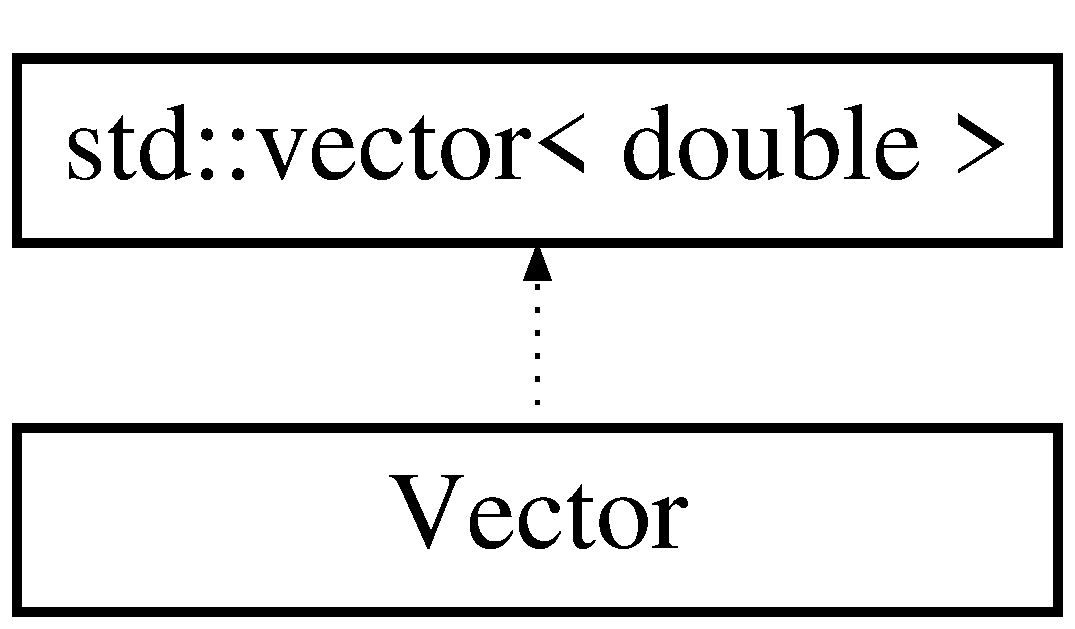
\includegraphics[height=2.000000cm]{classVector}
\end{center}
\end{figure}
\subsection*{Public Member Functions}
\begin{DoxyCompactItemize}
\item 
\mbox{\hyperlink{classVector_a6f80c73b5f18dcf3f8e36065bdc8b9e5}{Vector}} ()
\item 
\mbox{\hyperlink{classVector_acbdf66550f2caa0a64e0b356fb63a277}{Vector}} (int Num)
\item 
\mbox{\hyperlink{classVector_a5f04e343b7306ad11f8a82c89b486764}{Vector}} (const \mbox{\hyperlink{classVector}{Vector}} \&v)
\item 
\mbox{\hyperlink{classVector}{Vector}} \& \mbox{\hyperlink{classVector_ae48c467a9f65d60e2f7455aba4ca1239}{operator=}} (const \mbox{\hyperlink{classVector}{Vector}} \&v)
\item 
bool \mbox{\hyperlink{classVector_ade5fbd0cd01b034d1907e0c93433320c}{operator==}} (const \mbox{\hyperlink{classVector}{Vector}} \&v) const
\item 
int \mbox{\hyperlink{classVector_afbb7966ec4107c43ec15cccc47fcaef7}{get\+Size}} () const
\item 
double \mbox{\hyperlink{classVector_a6752a90058ddef427ca6aed12946a737}{one\+\_\+norm}} () const
\item 
double \mbox{\hyperlink{classVector_a4f501290a50d057bb6c57ea64d7e70a4}{two\+\_\+norm}} () const
\item 
double \mbox{\hyperlink{classVector_a50b72131eaf3698a9876d99ab6912a32}{uniform\+\_\+norm}} () const
\end{DoxyCompactItemize}
\subsection*{Friends}
\begin{DoxyCompactItemize}
\item 
std\+::istream \& \mbox{\hyperlink{classVector_ac198cff0f4196c66649278458eebf227}{operator$>$$>$}} (std\+::istream \&is, \mbox{\hyperlink{classVector}{Vector}} \&v)
\item 
std\+::ostream \& \mbox{\hyperlink{classVector_ac254b27efeb8486ee2f67821e3a21a60}{operator$<$$<$}} (std\+::ostream \&os, const \mbox{\hyperlink{classVector}{Vector}} \&v)
\item 
std\+::ifstream \& \mbox{\hyperlink{classVector_ab6009b37fac65598b3db164dc4f19fed}{operator$>$$>$}} (std\+::ifstream \&ifs, \mbox{\hyperlink{classVector}{Vector}} \&v)
\item 
std\+::ofstream \& \mbox{\hyperlink{classVector_a8e755f5550c983df730602890058d990}{operator$<$$<$}} (std\+::ofstream \&ofs, const \mbox{\hyperlink{classVector}{Vector}} \&v)
\end{DoxyCompactItemize}


\subsection{Detailed Description}
A vector class for data storage of a 1D array of doubles ~\newline
 The implementation is derived from the standard container vector std\+::vector ~\newline
 We use private inheritance to base our vector upon the library version whilst  usto expose only those base class functions we wish to use -\/ in this  the array access operator \mbox{[}\mbox{]}

The \mbox{\hyperlink{classVector}{Vector}} class provides\+: ~\newline
-\/basic constructors for creating vector obcjet from other vector object, or by creating empty vector of a given size, ~\newline
-\/input and oput operation via $>$$>$ and $<$$<$ operators using keyboard or file ~\newline
-\/basic operations like access via \mbox{[}\mbox{]} operator, assignment and comparision 

\subsection{Constructor \& Destructor Documentation}
\mbox{\Hypertarget{classVector_a6f80c73b5f18dcf3f8e36065bdc8b9e5}\label{classVector_a6f80c73b5f18dcf3f8e36065bdc8b9e5}} 
\index{Vector@{Vector}!Vector@{Vector}}
\index{Vector@{Vector}!Vector@{Vector}}
\subsubsection{\texorpdfstring{Vector()}{Vector()}\hspace{0.1cm}{\footnotesize\ttfamily [1/3]}}
{\footnotesize\ttfamily Vector\+::\+Vector (\begin{DoxyParamCaption}{ }\end{DoxyParamCaption})}

Default constructor. Intialize an empty \mbox{\hyperlink{classVector}{Vector}} object \begin{DoxySeeAlso}{See also}
\mbox{\hyperlink{classVector_acbdf66550f2caa0a64e0b356fb63a277}{Vector(int Num)}} 

\mbox{\hyperlink{classVector_a5f04e343b7306ad11f8a82c89b486764}{Vector(const Vector\& v)}} 
\end{DoxySeeAlso}
\mbox{\Hypertarget{classVector_acbdf66550f2caa0a64e0b356fb63a277}\label{classVector_acbdf66550f2caa0a64e0b356fb63a277}} 
\index{Vector@{Vector}!Vector@{Vector}}
\index{Vector@{Vector}!Vector@{Vector}}
\subsubsection{\texorpdfstring{Vector()}{Vector()}\hspace{0.1cm}{\footnotesize\ttfamily [2/3]}}
{\footnotesize\ttfamily Vector\+::\+Vector (\begin{DoxyParamCaption}\item[{int}]{Num }\end{DoxyParamCaption})\hspace{0.3cm}{\ttfamily [explicit]}}

Explicit alterative constructor takes an intiger. it is explicit since implicit type conversion int -\/$>$ vector doesn\textquotesingle{}t make sense Intialize \mbox{\hyperlink{classVector}{Vector}} object of size Num \begin{DoxySeeAlso}{See also}
\mbox{\hyperlink{classVector_a6f80c73b5f18dcf3f8e36065bdc8b9e5}{Vector()}} 

\mbox{\hyperlink{classVector_a5f04e343b7306ad11f8a82c89b486764}{Vector(const Vector\& v)}} 
\end{DoxySeeAlso}

\begin{DoxyExceptions}{Exceptions}
{\em invalid\+\_\+argument} & (\char`\"{}vector size negative\char`\"{}) \\
\hline
\end{DoxyExceptions}

\begin{DoxyParams}{Parameters}
{\em Num} & int. Size of a vector \\
\hline
\end{DoxyParams}
\mbox{\Hypertarget{classVector_a5f04e343b7306ad11f8a82c89b486764}\label{classVector_a5f04e343b7306ad11f8a82c89b486764}} 
\index{Vector@{Vector}!Vector@{Vector}}
\index{Vector@{Vector}!Vector@{Vector}}
\subsubsection{\texorpdfstring{Vector()}{Vector()}\hspace{0.1cm}{\footnotesize\ttfamily [3/3]}}
{\footnotesize\ttfamily Vector\+::\+Vector (\begin{DoxyParamCaption}\item[{const \mbox{\hyperlink{classVector}{Vector}} \&}]{v }\end{DoxyParamCaption})}

Copy constructor takes an \mbox{\hyperlink{classVector}{Vector}} object reference. Intialize \mbox{\hyperlink{classVector}{Vector}} object with another \mbox{\hyperlink{classVector}{Vector}} object \begin{DoxySeeAlso}{See also}
\mbox{\hyperlink{classVector_a6f80c73b5f18dcf3f8e36065bdc8b9e5}{Vector()}} 

\mbox{\hyperlink{classVector_acbdf66550f2caa0a64e0b356fb63a277}{Vector(int Num)}} 
\end{DoxySeeAlso}


\subsection{Member Function Documentation}
\mbox{\Hypertarget{classVector_afbb7966ec4107c43ec15cccc47fcaef7}\label{classVector_afbb7966ec4107c43ec15cccc47fcaef7}} 
\index{Vector@{Vector}!get\+Size@{get\+Size}}
\index{get\+Size@{get\+Size}!Vector@{Vector}}
\subsubsection{\texorpdfstring{get\+Size()}{getSize()}}
{\footnotesize\ttfamily int Vector\+::get\+Size (\begin{DoxyParamCaption}{ }\end{DoxyParamCaption}) const}

Normal get method that returns integer, the size of the vector \begin{DoxyReturn}{Returns}
int. the size of the vector 
\end{DoxyReturn}
\mbox{\Hypertarget{classVector_a6752a90058ddef427ca6aed12946a737}\label{classVector_a6752a90058ddef427ca6aed12946a737}} 
\index{Vector@{Vector}!one\+\_\+norm@{one\+\_\+norm}}
\index{one\+\_\+norm@{one\+\_\+norm}!Vector@{Vector}}
\subsubsection{\texorpdfstring{one\+\_\+norm()}{one\_norm()}}
{\footnotesize\ttfamily double Vector\+::one\+\_\+norm (\begin{DoxyParamCaption}{ }\end{DoxyParamCaption}) const}

Normal public method that returns a double. It returns L1 norm of vector \begin{DoxySeeAlso}{See also}
\mbox{\hyperlink{classVector_a4f501290a50d057bb6c57ea64d7e70a4}{two\+\_\+norm()const}} 

\mbox{\hyperlink{classVector_a50b72131eaf3698a9876d99ab6912a32}{uniform\+\_\+norm()const}} 
\end{DoxySeeAlso}
\begin{DoxyReturn}{Returns}
double. vectors L1 norm 
\end{DoxyReturn}
\mbox{\Hypertarget{classVector_ae48c467a9f65d60e2f7455aba4ca1239}\label{classVector_ae48c467a9f65d60e2f7455aba4ca1239}} 
\index{Vector@{Vector}!operator=@{operator=}}
\index{operator=@{operator=}!Vector@{Vector}}
\subsubsection{\texorpdfstring{operator=()}{operator=()}}
{\footnotesize\ttfamily \mbox{\hyperlink{classVector}{Vector}} \& Vector\+::operator= (\begin{DoxyParamCaption}\item[{const \mbox{\hyperlink{classVector}{Vector}} \&}]{v }\end{DoxyParamCaption})}

Overloaded assignment operator \begin{DoxySeeAlso}{See also}
\mbox{\hyperlink{classVector_ade5fbd0cd01b034d1907e0c93433320c}{operator==(const Vector\& v)const}} 
\end{DoxySeeAlso}

\begin{DoxyParams}{Parameters}
{\em v} & \mbox{\hyperlink{classVector}{Vector}} to assign from \\
\hline
\end{DoxyParams}
\begin{DoxyReturn}{Returns}
the object on the left of the assignment 
\end{DoxyReturn}

\begin{DoxyParams}{Parameters}
{\em v} & Vecto\&. \mbox{\hyperlink{classVector}{Vector}} to assign from \\
\hline
\end{DoxyParams}
\mbox{\Hypertarget{classVector_ade5fbd0cd01b034d1907e0c93433320c}\label{classVector_ade5fbd0cd01b034d1907e0c93433320c}} 
\index{Vector@{Vector}!operator==@{operator==}}
\index{operator==@{operator==}!Vector@{Vector}}
\subsubsection{\texorpdfstring{operator==()}{operator==()}}
{\footnotesize\ttfamily bool Vector\+::operator== (\begin{DoxyParamCaption}\item[{const \mbox{\hyperlink{classVector}{Vector}} \&}]{v }\end{DoxyParamCaption}) const}

Overloaded comparison operator returns true if vectors are the same within a tolerance (1.\+e-\/07) \begin{DoxySeeAlso}{See also}
\mbox{\hyperlink{classVector_ae48c467a9f65d60e2f7455aba4ca1239}{operator=(const Vector\& v)}} 

operator\mbox{[}$\,$\mbox{]}(int i) 

operator\mbox{[}$\,$\mbox{]}(int i)const 
\end{DoxySeeAlso}
\begin{DoxyReturn}{Returns}
bool. true or false 
\end{DoxyReturn}

\begin{DoxyExceptions}{Exceptions}
{\em invalid\+\_\+argument} & (\char`\"{}incompatible vector sizes\textbackslash{}n\char`\"{}) \\
\hline
\end{DoxyExceptions}

\begin{DoxyParams}{Parameters}
{\em v} & \mbox{\hyperlink{classVector}{Vector}}\&. vector to compare \\
\hline
\end{DoxyParams}
\mbox{\Hypertarget{classVector_a4f501290a50d057bb6c57ea64d7e70a4}\label{classVector_a4f501290a50d057bb6c57ea64d7e70a4}} 
\index{Vector@{Vector}!two\+\_\+norm@{two\+\_\+norm}}
\index{two\+\_\+norm@{two\+\_\+norm}!Vector@{Vector}}
\subsubsection{\texorpdfstring{two\+\_\+norm()}{two\_norm()}}
{\footnotesize\ttfamily double Vector\+::two\+\_\+norm (\begin{DoxyParamCaption}{ }\end{DoxyParamCaption}) const}

Normal public method that returns a double. It returns L2 norm of vector \begin{DoxySeeAlso}{See also}
\mbox{\hyperlink{classVector_a6752a90058ddef427ca6aed12946a737}{one\+\_\+norm()const}} 

\mbox{\hyperlink{classVector_a50b72131eaf3698a9876d99ab6912a32}{uniform\+\_\+norm()const}} 
\end{DoxySeeAlso}
\begin{DoxyReturn}{Returns}
double. vectors L2 norm 
\end{DoxyReturn}
\mbox{\Hypertarget{classVector_a50b72131eaf3698a9876d99ab6912a32}\label{classVector_a50b72131eaf3698a9876d99ab6912a32}} 
\index{Vector@{Vector}!uniform\+\_\+norm@{uniform\+\_\+norm}}
\index{uniform\+\_\+norm@{uniform\+\_\+norm}!Vector@{Vector}}
\subsubsection{\texorpdfstring{uniform\+\_\+norm()}{uniform\_norm()}}
{\footnotesize\ttfamily double Vector\+::uniform\+\_\+norm (\begin{DoxyParamCaption}{ }\end{DoxyParamCaption}) const}

Normal public method that returns a double. It returns L\+\_\+max norm of vector \begin{DoxySeeAlso}{See also}
\mbox{\hyperlink{classVector_a6752a90058ddef427ca6aed12946a737}{one\+\_\+norm()const}} 

\mbox{\hyperlink{classVector_a4f501290a50d057bb6c57ea64d7e70a4}{two\+\_\+norm()const}} 
\end{DoxySeeAlso}

\begin{DoxyExceptions}{Exceptions}
{\em out\+\_\+of\+\_\+range} & (\char`\"{}vector access error\char`\"{}) vector has zero size \\
\hline
\end{DoxyExceptions}
\begin{DoxyReturn}{Returns}
double. vectors Lmax norm 
\end{DoxyReturn}


\subsection{Friends And Related Function Documentation}
\mbox{\Hypertarget{classVector_ac254b27efeb8486ee2f67821e3a21a60}\label{classVector_ac254b27efeb8486ee2f67821e3a21a60}} 
\index{Vector@{Vector}!operator$<$$<$@{operator$<$$<$}}
\index{operator$<$$<$@{operator$<$$<$}!Vector@{Vector}}
\subsubsection{\texorpdfstring{operator$<$$<$}{operator<<}\hspace{0.1cm}{\footnotesize\ttfamily [1/2]}}
{\footnotesize\ttfamily std\+::ostream\& operator$<$$<$ (\begin{DoxyParamCaption}\item[{std\+::ostream \&}]{os,  }\item[{const \mbox{\hyperlink{classVector}{Vector}} \&}]{v }\end{DoxyParamCaption})\hspace{0.3cm}{\ttfamily [friend]}}

Overloaded ifstream $<$$<$ operator. Display output. \begin{DoxySeeAlso}{See also}
\mbox{\hyperlink{classVector_ac198cff0f4196c66649278458eebf227}{operator$>$$>$(std\+::istream\& is, Vector\& v)}} 

\mbox{\hyperlink{classVector_ab6009b37fac65598b3db164dc4f19fed}{operator$>$$>$(std\+::ifstream\& ifs, Vector\& v)}} 

\mbox{\hyperlink{classVector_a8e755f5550c983df730602890058d990}{operator$<$$<$(std\+::ofstream\& ofs, const Vector\& v)}} 
\end{DoxySeeAlso}
\begin{DoxyReturn}{Returns}
std\+::ostream\&. the output stream object os 
\end{DoxyReturn}

\begin{DoxyParams}{Parameters}
{\em os} & output file stream \\
\hline
{\em v} & vector to read from \\
\hline
\end{DoxyParams}
\mbox{\Hypertarget{classVector_a8e755f5550c983df730602890058d990}\label{classVector_a8e755f5550c983df730602890058d990}} 
\index{Vector@{Vector}!operator$<$$<$@{operator$<$$<$}}
\index{operator$<$$<$@{operator$<$$<$}!Vector@{Vector}}
\subsubsection{\texorpdfstring{operator$<$$<$}{operator<<}\hspace{0.1cm}{\footnotesize\ttfamily [2/2]}}
{\footnotesize\ttfamily std\+::ofstream\& operator$<$$<$ (\begin{DoxyParamCaption}\item[{std\+::ofstream \&}]{ofs,  }\item[{const \mbox{\hyperlink{classVector}{Vector}} \&}]{v }\end{DoxyParamCaption})\hspace{0.3cm}{\ttfamily [friend]}}

Overloaded ofstream $<$$<$ operator. File output. the file output operator is compatible with file input operator, ie. everything written can be read later. \begin{DoxySeeAlso}{See also}
\mbox{\hyperlink{classVector_ac198cff0f4196c66649278458eebf227}{operator$>$$>$(std\+::istream\& is, Vector\& v)}} 

\mbox{\hyperlink{classVector_ab6009b37fac65598b3db164dc4f19fed}{operator$>$$>$(std\+::ifstream\& ifs, Vector\& v)}} 

\mbox{\hyperlink{classVector_ac254b27efeb8486ee2f67821e3a21a60}{operator$<$$<$(std\+::ostream\& os, const Vector\& v)}} 
\end{DoxySeeAlso}
\begin{DoxyReturn}{Returns}
std\+::ofstream\&. the output ofstream object ofs 
\end{DoxyReturn}

\begin{DoxyParams}{Parameters}
{\em ofs} & outputfile stream. With opened file \\
\hline
{\em v} & \mbox{\hyperlink{classVector}{Vector}}\&. vector to read from \\
\hline
\end{DoxyParams}
\mbox{\Hypertarget{classVector_ac198cff0f4196c66649278458eebf227}\label{classVector_ac198cff0f4196c66649278458eebf227}} 
\index{Vector@{Vector}!operator$>$$>$@{operator$>$$>$}}
\index{operator$>$$>$@{operator$>$$>$}!Vector@{Vector}}
\subsubsection{\texorpdfstring{operator$>$$>$}{operator>>}\hspace{0.1cm}{\footnotesize\ttfamily [1/2]}}
{\footnotesize\ttfamily std\+::istream\& operator$>$$>$ (\begin{DoxyParamCaption}\item[{std\+::istream \&}]{is,  }\item[{\mbox{\hyperlink{classVector}{Vector}} \&}]{v }\end{DoxyParamCaption})\hspace{0.3cm}{\ttfamily [friend]}}

Overloaded istream $>$$>$ operator. Keyboard input if vector has size user will be asked to input only vector values if vector was not initialized user can choose vector size and input it values \begin{DoxySeeAlso}{See also}
\mbox{\hyperlink{classVector_ab6009b37fac65598b3db164dc4f19fed}{operator$>$$>$(std\+::ifstream\& ifs, Vector\& v)}} 

\mbox{\hyperlink{classVector_ac254b27efeb8486ee2f67821e3a21a60}{operator$<$$<$(std\+::ostream\& os, const Vector\& v)}} 

\mbox{\hyperlink{classVector_a8e755f5550c983df730602890058d990}{operator$<$$<$(std\+::ofstream\& ofs, const Vector\& v)}} 
\end{DoxySeeAlso}
\begin{DoxyReturn}{Returns}
std\+::istream\&. the input stream object is 
\end{DoxyReturn}

\begin{DoxyExceptions}{Exceptions}
{\em std\+::invalid\+\_\+argument} & (\char`\"{}read error -\/ negative vector size\char`\"{}); \\
\hline
\end{DoxyExceptions}

\begin{DoxyParams}{Parameters}
{\em is} & keyboard input straem. For user input \\
\hline
{\em v} & \mbox{\hyperlink{classVector}{Vector}}\&. vector to write to \\
\hline
\end{DoxyParams}
\mbox{\Hypertarget{classVector_ab6009b37fac65598b3db164dc4f19fed}\label{classVector_ab6009b37fac65598b3db164dc4f19fed}} 
\index{Vector@{Vector}!operator$>$$>$@{operator$>$$>$}}
\index{operator$>$$>$@{operator$>$$>$}!Vector@{Vector}}
\subsubsection{\texorpdfstring{operator$>$$>$}{operator>>}\hspace{0.1cm}{\footnotesize\ttfamily [2/2]}}
{\footnotesize\ttfamily std\+::ifstream\& operator$>$$>$ (\begin{DoxyParamCaption}\item[{std\+::ifstream \&}]{ifs,  }\item[{\mbox{\hyperlink{classVector}{Vector}} \&}]{v }\end{DoxyParamCaption})\hspace{0.3cm}{\ttfamily [friend]}}

Overloaded ifstream $>$$>$ operator. File input the file output operator is compatible with file input operator, ie. everything written can be read later. \begin{DoxySeeAlso}{See also}
\mbox{\hyperlink{classVector_ac198cff0f4196c66649278458eebf227}{operator$>$$>$(std\+::istream\& is, Vector\& v)}} 

\mbox{\hyperlink{classVector_ac254b27efeb8486ee2f67821e3a21a60}{operator$<$$<$(std\+::ostream\& os, const Vector\& v)}} 

\mbox{\hyperlink{classVector_a8e755f5550c983df730602890058d990}{operator$<$$<$(std\+::ofstream\& ofs, const Vector\& v)}} 
\end{DoxySeeAlso}
\begin{DoxyReturn}{Returns}
ifstream\&. the input ifstream object ifs 
\end{DoxyReturn}

\begin{DoxyExceptions}{Exceptions}
{\em std\+::invalid\+\_\+argument} & (\char`\"{}file read error -\/ negative vector size\char`\"{}); \\
\hline
\end{DoxyExceptions}

\begin{DoxyParams}{Parameters}
{\em ifs} & input file straem. With opened matrix file \\
\hline
{\em v} & \mbox{\hyperlink{classVector}{Vector}}\&. vector to write to \\
\hline
\end{DoxyParams}


The documentation for this class was generated from the following files\+:\begin{DoxyCompactItemize}
\item 
vector.\+h\item 
vector.\+cpp\end{DoxyCompactItemize}

%--- End generated contents ---

% Index
\backmatter
\newpage
\phantomsection
\clearemptydoublepage
\addcontentsline{toc}{chapter}{Index}
\printindex

\end{document}
